\documentclass[oneside]{book}

\usepackage[book]{dennis}
\RequirePackage{cover}

\title{Exploring Euclidean Geometry V2}
\author{Dennis Chen}
\date{\today}

\begin{document}

\usepackage{pstricks}
\usepackage{anyfontsize}
\definecolor{pink}{rgb}{1,0.7,0.7}
\definecolor{OliveGreen}{rgb}{0,0.6,0}
\definecolor{amaranth}{rgb}{0.9, 0.17, 0.31}

\usepackage[pages=some]{background}
\backgroundsetup{
scale=1,
color=black,
opacity=0.4,
angle=0,
contents={%
  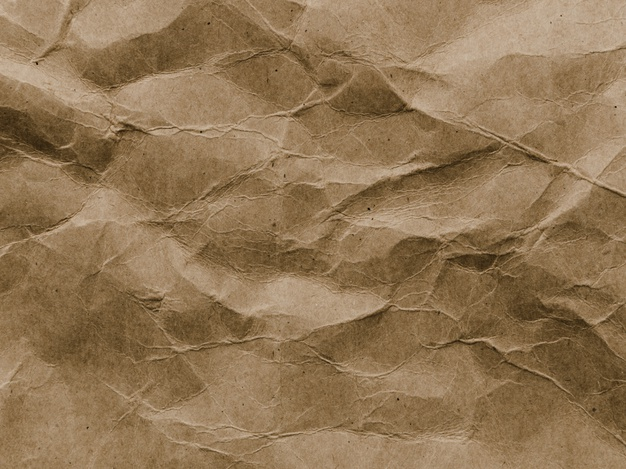
\includegraphics[width=\paperwidth,height=\paperheight]{crumpled-brown-paper.jpg}
  }%
}

\newtcolorbox{cross}{blank,breakable,parbox=false,
  overlay={\draw[red,line width=5pt] (interior.south west)--(interior.north east);
    \draw[red,line width=5pt] (interior.north west)--(interior.south east);}}

\maketitle

\section*{Introduction}
This is a preview of Exploring Euclidean Geometry V2. It contains the first five chapters, which constitute the entirety of the first part.

This should be a good introduction for those training for computational geometry questions. This book may be somewhat rough on beginners, so I do recommend using some slower-paced books as a supplement, but I believe the explanations should be concise and clear enough to understand. In particular, a lot of other texts have unnecessarily long proofs for basic theorems, while this book will try to prove it as clearly and succintly as possible.

There aren't a ton of worked examples in this section, but the check-ins should suffice since they're just direct applications of the material.

\pagebreak

\toc

\part{The Basics}

\chapter{Triangle Centers}

\chapterquote{Empty your mind of any theories,\\ 'Til all the facts are in.}{Death Note Musical}

We define the primary four triangle centers, their corresponding lines, and define a cevian.

\begin{defi}[Cevian]
In a triangle, a cevian is a line segment with a vertex of the triangle as an endpoint and its other endpoint on the opposite side.

\begin{center}
\begin{asy}
size(4cm);
dot((-1,0));
dot((-2,0));
dot((2,0));
dot((1,2));

draw((-2,0)--(2,0)--(1,2)--cycle);
draw((1,2)--(-1,0));

\end{asy}
\end{center}
\end{defi}

\section{Incenter}

The corresponding cevian is the \textit{interior} angle bisector.

\begin{defi}[Interior Angle Bisector]
The interior angle bisector of $\angle CAB$ is the line that bisects acute $\angle CAB.$
\end{defi}

The interior angle bisector of $\angle CAB$ is also the locus of points inside $\angle CAB$ equidistant from lines $AB$ and $AC.$

\begin{fact}[Angle Bisector Equidistant from Both Sides]
In $\angle CAB,$ $\angle PAB=\angle PAC$ if and only if $\delta(P,AB)=\delta(P,AC).$
\end{fact}

\begin{pro}
Let the feet of the altitudes from $P$ to $AB,AC$ be $X,Y.$ Then note that either of these conditions imply $\triangle APX\cong \triangle APY,$ which in turn implies the other condition.
\end{pro}

\begin{theo}[Incenter]
There is a point $I$ that the angle bisectors of $\triangle ABC$ concur at. Furthermore, $I$ is equidistant from sides $AB,BC,CA.$
\end{theo}

\begin{pro}
Recall that a point is on the angle bisector of $\angle CAB$ if and only if $\delta(P,AB)=\delta(P,AC).$ Let the angle bisectors of $\angle CAB$ and $\angle ABC$ intersect at $I.$ Then $\delta(P,CA)=\delta(P,AB)$ and $\delta(P,AB)=\delta(P,BC),$ so $\delta(P,BC)=\delta(P,CA),$ implying that $I$ lies on the angle bisector of $\angle BCA.$

Since $\delta(P,AB)=\delta(P,BC)=\delta(P,CA),$ the circle with radius $\delta(P,AB)$ centered at $I$ is inscribed in $\triangle ABC.$
\begin{center}
    \begin{asy}
import olympiad;
    size(4cm);
    pair A=dir(110);
    pair B=dir(210);
    pair C=dir(-30),D,E,F,I;
    I=incenter(A,B,C);
    D=foot(I,B,C);
    E=foot(I,C,A);
    F=foot(I,A,B);
    dot(A^^B^^C^^I^^D^^E^^F);
    draw(incircle(A,B,C),blue);
    draw(A--B--C--cycle);
    draw(A--I--B);
    draw(I--C,red);
    draw(I--D,dotted);
    draw(I--E,dotted);
    draw(I--F,dotted);
    label("A",A,dir(90));
    label("B",B,dir(200));
    label("C",C,dir(-20));
    label("D",D,dir(-90));
    label("E",E,dir(35));
    label("F",F,dir(135));
    label("I",I,dir(60));
    \end{asy}
\end{center}
\end{pro}

\section{Centroid}

The corresponding cevian is the median.

\begin{defi}[Midpoint]
The midpoint of segment $AB$ is the unique point $M$ that satisfies the following:
\begin{enumerate}[label=(\alph*)]
    \item $M$ is on $AB.$
    
    \item $AM=MB.$
\end{enumerate}
\end{defi}

\begin{defi}[Median]
The $A$-median of $\triangle ABC$ is the line segment that joins $A$ with the midpoint of $BC.$
\end{defi}

\begin{theo}[Centroid]
The medians $AD,BE,CF$ of $\triangle ABC$ concur at a point $G.$ Furthermore, the following two properties hold:
\begin{enumerate}[label=(\alph*)]
    \item $\frac{AG}{GD}=\frac{BG}{GE}=\frac{CG}{GF}=2.$
    
    \item $[BGD]=[CGD]=[CGE]=[AGE]=[AGF]=[BGF].$
\end{enumerate}

\end{theo}

\begin{pro}
Let $BE$ intersect $CF$ at $G.$ Since $\triangle AFE\sim \triangle ABC,$ $FE\parallel BC.$ Thus $\triangle BCG\sim\triangle EFG$ with a ratio of $\frac{BC}{EF}=2,$ so $\frac{BG}{GE}=2.$

Similarly let $BE$ intersect $AD$ at $G'.$ Repeating the above yields $\frac{BG'}{G'E}=2.$ Thus $G$ and $G'$ are the same point, and the medians are concurrent.

\begin{center}
    \begin{asy}
    import olympiad;
    size(5cm);
    pair A=dir(110), B=dir(200), C=dir(-20), D,E,F,G;
    G=(A+B+C)/3;
    D=(B+C)/2;
    E=(C+A)/2;
    F=(A+B)/2;
    dot(A^^B^^C^^D^^E^^F^^G);
    draw(A--B--C--A);
    draw(E--F);
    draw(B--E);
    draw(C--F);
    label("A",A,N);
    label("B",B,dir(190));
    label("C",C,dir(-10));
    label("D",D,S);
    label("E",E,dir(45));
    label("F",F,dir(140));
    label("G",G,dir(90));
    \end{asy}
\end{center}
\end{pro}

\begin{exam}[JMC 10 2020/20]
Consider triangle $ABC$ with medians $\overline{BE}$ and $\overline{CF}$ that intersect at $G.$ If $AG=BC=8$ and $CG=6,$ what is the length of $\overline{GE}$?
\end{exam}

\begin{sol}
The key step is to realize that $\angle{BGC}$ is right. We can prove this in two ways.

The first way is let $\overline{AG}$ meet $\overline{BC}$ at point $P$. The length of $\overline{PG}$ is $\tfrac{8}{2} = 4$. So $BP = PG = PC = 4$ and $\triangle{BGC}$ can be circumscribed in a circle with diameter $\overline{BC}$. It follows that $\angle{BGC} = 90^{\circ}$. 

The second way is to extend point $P$ to meet $\overline{GC}$ at midpoint $M$. Since $\triangle{GPC}$ is isosceles, $PG = PC$. We also have $BP = PC$ and $\angle{PMC} = 90^{\circ}$. $\triangle{PMC} \sim \triangle{BGC}$ by side-angle-side and the rest follows.

By the Pythagorean theorem, $\overline{BG}$ has length $2\sqrt{7} \Rightarrow GE = \tfrac{2\sqrt{7}}{2} = \boxed{\sqrt{7}}$.

    \begin{figure}[h!]
        \centering
        \begin{asy}
        size(4cm);
        fill((0,0)--(7/2,3sqrt(7)/2)--(8,0)--cycle,rgb(230,255,242));
        dot((0,0));
        dot((8,0));
        label("$B$",(0,0), SW);
        label("$P$",(4,0), S);
        label("$G$",(7/2,(3sqrt(7))/2),NW);
        label("$C$",(8,0), SE);
        label("$A$",(5/2,9sqrt(7)/2), N);
        label("$E$",(21/4,9sqrt(7)/4), NE);
        dot((7/2,(3sqrt(7))/2));
        dot((5/2,(9sqrt(7))/2));
        draw((0,0)--(8,0)--(5/2,(9sqrt(7))/2)--(0,0));
        draw((5/2,(9sqrt(7))/2)--(4,0));
        draw((7/2,(3sqrt(7))/2)--(8,0));
        draw((0,0)..(7/2,(3sqrt(7))/2)..(8,0)..(9/2,(-3sqrt(7))/2)..(0,0), dotted);
        draw((0,0)--(7/2,(3sqrt(7))/2));
        draw((7/2,(3sqrt(7))/2)--(21/4,(9sqrt(7))/4));
        \end{asy}
    \end{figure}
\end{sol}

\section{Circumcenter}

A perpendicular bisector is not a cevian, but it is still a special line in triangles.

\begin{defi}[Perpendicular Bisector]
The perpendicular bisector of a line segment $AB$ is the locus of points $X$ such that $AX=BX.$
\end{defi}

The circumcenter is the unique circle that contains points $A,B,C.$

\begin{theo}[Circumcenter]
There is a point $O$ that the perpendicular bisectors of $BC,CA,AB$ concur at. Furthermore, $O$ is the center of $(ABC).$
\end{theo}

\begin{pro}
Let the perpendicular bisectors of $AB,BC$ intersect at $O.$ By the definition of a perpendicular bisector, $AO=BO$ and $BO=CO.$ But this implies $CO=AO,$ so $O$ lies on the perpendicular bisector of $CA.$

Since $AO=BO=CO,$ the circle centered at $O$ with radius $AO$ circumscribes $\triangle ABC.$

\begin{center}
    \begin{asy}
    import olympiad;
    size(4cm);
    pair A=dir(110);
    pair B=dir(210);
    pair C=dir(-30),D,E,F,I;
    I=circumcenter(A,B,C);
    D=foot(I,B,C);
    E=foot(I,C,A);
    F=foot(I,A,B);
    dot(A^^B^^C^^I^^D^^E^^F);
    draw(circumcircle(A,B,C),blue);
    draw(A--B--C--cycle);
    draw(A--I--B,dotted);
    draw(I--C,dotted);
    draw(I--D);
    draw(I--E,red);
    draw(I--F);
    label("A",A,dir(90));
    label("B",B,dir(200));
    label("C",C,dir(-20));
    label("D",D,dir(-90));
    label("E",E,dir(35));
    label("F",F,dir(135));
    label("O",I,dir(95));
    \end{asy}
\end{center}
\end{pro}

\section{Orthocenter}

The corresponding cevian is the altitude.

\begin{defi}[Altitude]
The $A$-altitude of $\triangle ABC$ is the line through $A$ perpendicular to $BC.$
\end{defi}

\begin{defi}[Foot of Altitude]
The foot of the altitude from $A$ to $BC$ is the point $H$ where the $A$-altitude intersects $BC.$
\end{defi}

\begin{theo}[Orthocenter]
The altitudes of $\triangle ABC$ concur.
\end{theo}

\begin{pro}
We will be piggybacking on the proof for the circumcenter.

Let the line through $B$ parallel to $AC$ and the line through $C$ parallel to $AB$ intersect at $D.$ Define $E,F$ similarly. Note that $FA=BC=AE,$ so the $A$ altitude of $\triangle ABC$ is the perpendicular bisector of $DE.$ Since the circumcenter exists, the orthocenter must too.

\begin{center}
    \begin{asy}
    import olympiad;
    size(4cm);
    pair A=dir(110), B=dir(200), C=dir(-20), D,E,F,H;
    H=orthocenter(A,B,C);
    D=B+C-A;
    E=C+A-B;
    F=A+B-C;
    dot(A^^B^^C^^D^^E^^F^^H);
    draw(A--B--C--A);
    draw(D--E--F--D);
    draw(A--H,dotted);
    draw(B--H,dotted);
    draw(C--H,dotted);
    label("A",A,N);
    label("B",B,dir(190));
    label("C",C,dir(-10));
    label("D",D,S);
    label("E",E,dir(45));
    label("F",F,dir(140));
    label("H",H,dir(35));
    \end{asy}
\end{center}
\end{pro}

\section{Summary}

\subsection{Theory}

\begin{enumerate}
\item Angle Bisector
\begin{itemize}
\Item The angle bisector bisects the angle, as the name suggests.

\Item It is also the locus of points equidistant from two lines.
\end{itemize}

\item Incenter
\begin{itemize}
\Item The incenter is the center of the incircle.

\Item The incenter is equidistant from all sides.

\Item The incenter is the concurrence point of the angle bisectors.
\end{itemize}

\item Median
\begin{itemize}
\Item The median joins the vertex to the midpoint of the opposite side.
\end{itemize}

\item Centroid
\begin{itemize}
\Item The centroid is the center of mass.

\Item The centroid is the concurrence point of the medians.

\Item The centroid $G$ splits the medians in the ratio $\frac{AG}{GD}=2$.
\end{itemize}

\item Perpendicular Bisector
\begin{itemize}
\Item The perpendicular bisector is the locus of points equidistant from the endpoints of a line segment.

\Item The perpendicular bisector perpendicularly bisects the segment.
\end{itemize}

\item Circumcenter
\begin{itemize}
\Item The circumcenter is the center of the circumcircle.

\Item The circumcenter is equidistant from all vertices.

\Item The circumcenter is the concurrence point of the perpendicular bisectors.
\end{itemize}

\item Altitude
\begin{itemize}
\Item The altitude is the perpendicular line through one vertex to the opposite side.

\Item The foot of the altitude is the intersection of the altitude with the side.
\end{itemize}

\item Orthocenter
\begin{itemize}
\Item The orthocenter is the concurrence point of the altitudes.
\end{itemize}
\end{enumerate}

\subsection{Tips and Strategies}

\begin{enumerate}
\item Incenter
\begin{itemize}
\Item Just remember that the angle bisector bisects angles.
\end{itemize}

\item Centroid
\begin{itemize}
\Item Length chase with the length condition.

\Item Take homotheties from the midpoint of a side with scale factor $\frac{1}{3}$ to send the opposite vertex to the centroid.

\Item Remember that the medians split the triangle into six triangles of equal area.
\end{itemize}

\item Circumcenter
\begin{itemize}
\Item Use $AO=BO=CO$ to find isosceles triangles - this will help a lot with angle chasing.
\end{itemize}

\item Orthocenter
\begin{itemize}
\Item Watch out for right triangles and right angles.
\end{itemize}
\end{enumerate}

\pagebreak

\section{Exercises}

\subsection{Check-ins}

\begin{enumerate}
    \item Prove that a triangle is equilateral if and only if its incenter is the same point as its circumcenter.
    
    \item Consider $\triangle ABC$ with incenter $I.$ Prove that $\angle BIC=90^{\circ}+\frac{1}{2}\angle BAC.$
    \begin{hint}
    \begin{addhint}
    {Look at $\triangle BIC.$}
    \end{addhint}
    \end{hint}
    
    \item Prove that the perpendicular bisector of line segment $AB$ is perpendicular to and bisects $AB,$ if the perpendicular bisector is defined as the locus of points $X$ such that $AX=BX.$
    
    \item Consider $\triangle ABC$ with circumcenter $O.$ If $AO=20$ and $BC=32,$ find $[BOC].$
    
    \item (AMC 10A 2020/12) Triangle $AMC$ is isosceles with $AM = AC$. Medians $\overline{MV}$ and $\overline{CU}$ are perpendicular to each other, and $MV=CU=12$. What is the area of $\triangle AMC?$
    
    \begin{center}
        \begin{asy}
import olympiad;
size(4cm);
draw((-4,0)--(4,0)--(0,12)--cycle);
draw((-2,6)--(4,0));
draw((2,6)--(-4,0));
label("M", (-4,0), W);
label("C", (4,0), E);
label("A", (0, 12), N);
label("V", (2, 6), NE);
label("U", (-2, 6), NW);
label("P", (0, 3.6), S);
\end{asy}
    \end{center}
    
    \item Find the inradius and circumradius of an equilateral triangle with side length $x.$
\end{enumerate}

\subsection{Problems}

\begin{enumerate}
	\item (AMC 10B 2018/12) Line segment $\overline{AB}$ is a diameter of a circle with $AB=24$. Point $C$, not equal to $A$ or $B$, lies on the circle. As point $C$ moves around the circle, the centroid (center of mass) of $\triangle{ABC}$ traces out a closed curve missing two points. To the nearest positive integer, what is the area of the region bounded by this curve?
\begin{solu}
\begin{addsol}
{Let $O$ be the center of the circle and $G$ be the centroid of $\triangle ABC.$ Since $O$ is also the midpoint of $AB$ and thus lies on $CG$, we're motivated to make use of the $2:1$ ratio. $CO$ always has length $12,$ so it follows that $GO$ always has length $4.$ This means that the locus of $G$ is a circle with center $O$ and radius $4$ by definition, so the area is $16\pi\approx 50.$

\begin{center}
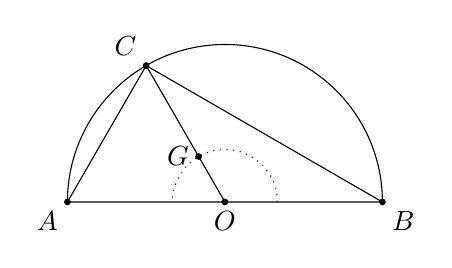
\begin{tikzpicture}
\draw (0,0)--(4,0)--(1,1.73205081)--cycle;
\draw (1,1.73205081)--(2,0);
\filldraw (0,0) circle (1pt) node[anchor= north east] {$A$};
\filldraw (4,0) circle (1pt) node[anchor=north west] {$B$};
\filldraw (1,1.73205081) circle (1pt) node[anchor=south east] {$C$};
\filldraw (2,0) circle (1pt) node[anchor= north] {$O$};
\filldraw (1.66666,0.57735027) circle (1pt) node[anchor= east] {$G$};
\draw (4,0) arc (0:180:2);
\draw[dotted] (8/3,0) arc (0:180:2/3);
\end{tikzpicture}
\end{center}}
\end{addsol}
\end{solu}

	\item Let $\triangle ABC$ have medians $BM,CN,$ and let $P$ and $Q$ be the feet of the altitudes from $B,C$ to $CN,BM,$ respectively. Prove that the quadrilateral $MNPQ$ is cyclic.
	\begin{hint}
	\begin{addhint}
	{Use Power of a Point.}
	\end{addhint}
	\begin{addhint}
	{Show that $GP\cdot GN=GQ\cdot GM,$ where $G$ is the centroid of $\triangle ABC.$}
	\end{addhint}
	\begin{addhint}
	{Remember that the centroid splits the median in a fixed ratio.}
	\end{addhint}
	\end{hint}
	\begin{solu}
	\begin{addsol}
	{Let the centroid be $G.$ We want to prove that $XP\cdot XN=XQ\cdot XM,$ which is equivalent to proving $XP\cdot XC=XQ\cdot XB,$ as $\frac{XC}{XN}=\frac{XB}{XM}=2.$ Now note that $BPQC$ is cyclic as $\angle BPC=\angle BQC=90^{\circ},$ which finishes the problem.}
	\end{addsol}
	\end{solu}

    \item Consider $\triangle ABC$ with medians $BE,CF.$ If $BE$ and $CF$ are perpendicular, find $\frac{b^2+c^2}{a^2}.$\begin{hint}
    \begin{addhint}
    {Look at $\triangle GBC.$}
    \end{addhint}
    \begin{addhint}
    {You can get $BE$ and $BF$ (via Stewart's), so you can get $BG$ and $CG.$}
    \end{addhint}
    \end{hint}
    \begin{solu}
    \begin{addsol}
    {By Stewart's, $BE=\frac{\sqrt{2c^2+2a^2-b^2}}{2}$ and $CF=\frac{\sqrt{2a^2+2b^2-c^2}}{2},$ so $a^2=BG^2+CF^2=\frac{4}{9}(\frac{2c^2+2a^2-b^2}{4}+\frac{2a^2+2b^2-c^2}{4})=\frac{4a^2+b^2+c^2}{9}.$
    
    Thus, $5a^2=b^2+c^2$ and $\frac{b^2+c^2}{a^2}=5.$}
    \end{addsol}
    \end{solu}
    
    \item (Brazil 2007) Let $ABC$ be a triangle with circumcenter $O$. Let $P$ be the intersection of straight lines $BO$ and $AC$ and $\omega$ be the circumcircle of triangle $AOP$. Suppose that $BO = AP$ and that the measure of the arc $OP$ in $\omega$, that does not contain $A$, is $40^{\circ}$. Determine the measure of the angle $\angle OBC$.
    \begin{hint}
    \begin{addhint}
    {Note that $BO=AO.$}
    \end{addhint}
    \begin{addhint}
    {$\triangle AOP$ is isosceles.}
    \end{addhint}
    \end{hint}
    \begin{solu}
    \begin{addsol}
    {Note that $BO=AO=AP,$ so $\triangle AOP$ is isosceles. Thus $\angle OAP=20^{\circ},$ implying $\angle AOC=140^{\circ},$ and $\angle AOP=\angle APO=80^{\circ},$ implying that $\angle AOB=100^{\circ}.$ So $\angle OBC=360^{\circ}-140^{\circ}-100^{\circ}=120^{\circ},$ or $\angle OBC=30^{\circ}.$
    
    \begin{center}
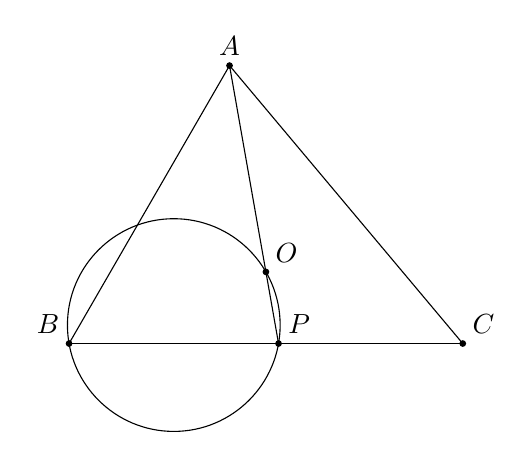
\begin{tikzpicture}
\draw (0.,0.)-- (5.,0.);
\draw (2.038018672739762,3.529951887959356)-- (0.,0.);
\draw (2.660444431189779,0.)-- (2.038018672739762,3.529951887959356);
\draw (2.038018672739762,3.529951887959356)-- (5.,0.);
\draw (1.3302222155948895,0.23455406694717237) circle (1.3507430374366678cm);

\filldraw (0.,0.) circle (1pt) node[anchor=south east] {$B$};
\filldraw (5.,0.) circle (1pt) node[anchor=south west] {$C$};
\filldraw (2.038018672739762,3.529951887959356) circle (1pt) node[anchor=south] {$A$};
\filldraw (2.5,0.9099255856655059) circle (1pt) node[anchor=south west] {$O$};
\filldraw (2.660444431189779,0.) circle (1pt) node[anchor=south west] {$P$};
\end{tikzpicture}
    \end{center}}
    \end{addsol}
    \end{solu}
\end{enumerate}

\subsection{Challenges}

\begin{enumerate}
    \item Three congruent circles $\omega_1,\omega_2,\omega_3$ concur at $P.$ Let $\omega_1$ intersect $\omega_2$ at $A\neq P,$ let $\omega_2$ intersect $\omega_3$ at $B\neq P,$ and let $\omega_3$ intersect $\omega_1$ at $C\neq P.$ What triangle center is $P$ with respect to $\triangle ABC?$
    
    \item Let $ABC$ be an isosceles triangle with $AB=AC.$ If $\omega$ is inscribed in $ABC$ and the orthocenter of $ABC$ lies on $\omega,$ find $\frac{AB}{BC}.$

    \item Let $G$ be the centroid of $\triangle ABC.$ If $\angle BGC=90^{\circ},$ find the maximum value $\sin A$ can take.
    \begin{hint}
    \begin{addhint}
    {Have you found $\frac{b^2+c^2}{a^2}$ yet?}
    \end{addhint}
    \end{hint}
\end{enumerate}

\chapter{Angle Chasing}

\chapterquote{'Think simple' as my old master used to say — meaning reduce the whole of its parts into the simplest terms, getting back to first principles.}{Frank Lloyd Wright}

You can angle chase to show points are collinear or lines are concurrent, lines are parallel, a line is tangent to a circle, or four points are cyclic. In computational contests, you may be asked to find an angle for easier problems and angle chasing can reveal more about the configuration for harder problems.

\section{Collinearity and Concurrency}

\begin{fact}[Collinearity Condition]
A line has measure $180^{\circ}.$ This means $A,B,C,$ are collinear if and only if for any point $P,$ $\angle ABP+\angle PBC=180^{\circ}.$ This is one of the main ways to prove points are collinear.
\end{fact}

\begin{center}
    \begin{asy}
    size(3.5cm);
    dot((0,0));
    dot((-1,0));
    dot((1,0));
    dot((-0.3,0.6));
    draw(arc((0,0),0.2,0,180));
    draw((-1,0)--(1,0));
    draw((0,0)--(-0.3,0.6));
    
    label("$A$",(-1,0),S);
    label("$B$",(0,0),S);
    label("$C$",(1,0),S);
    label("$P$",(-0.3,0.6),NW); 
    \end{asy}
\end{center}

This holds for more than one point too. For the right configuration, $A,B,C$ are collinear if and only if for points $P_1,P_2,\ldots,P_n,$ $\angle ABP_1+\angle P_1BP_2+\cdots+\angle P_nBC=180^{\circ}.$ (Directed angles can be used to avoid configuration issues.)

\begin{center}
    \begin{asy}
    size(3.5cm);
    dot((0,0));
    dot((-1,0));
    dot((1,0));
    dot((-0.3,0.6));
    dot((0.2,0.4));
    draw(arc((0,0),0.2,0,180));
    draw((-1,0)--(1,0));
    draw((0,0)--(-0.3,0.6));
    draw((0,0)--(0.2,0.4));
    
    label("$A$",(-1,0),S);
    label("$B$",(0,0),S);
    label("$C$",(1,0),S);
    label("$P_1$",(-0.3,0.6),NW);
    label("$P_2$",(0.2,0.4),NE);
    \end{asy}
\end{center}

A similar condition is that $A,B,C$ are collinear if and only if for any point $P,$ $\angle PAB=\angle PAC.$

\begin{center}
    \begin{asy}
    size(3.5cm);
    dot((0,0));
    dot((-1,0));
    dot((1,0));
    dot((-1.3,0.6));
    draw(arc((-1,0),0.2,0,120));
    draw((-1,0)--(1,0));
    draw((-1,0)--(-1.3,0.6));
    
    label("$A$",(-1,0),S);
    label("$B$",(0,0),S);
    label("$C$",(1,0),S);
    label("$P$",(-1.3,0.6),NW); 
    \end{asy}
\end{center}

\section{Parallel Lines}

\begin{fact}[Parallel Lines]
Consider parallel lines $AB$ and $CD.$ Then for $X$ on segment $AB$ and $Y$ on segment $CD,$
\[\angle AXY=180^{\circ}-\angle CYX=\angle DYX.\]
\end{fact}

\begin{center}
    \begin{asy}
    size(4cm);
    dot((-1,2));
    dot((3,6));
    dot((-5,-2));
    
    dot((1,-2));
    dot((5,2));
    dot((-3,-6));
    
    draw((-5,-2)--(3,6));
    draw((5,2)--(-3,-6));
    draw((1,-2)--(-1,2));
    
    draw(arc((1,-2),1,45,180-180atan(2)/pi));
    draw(arc((1,-2),0.9,180-180atan(2)/pi,225));
    draw(arc((-1,2),1,-135,180atan(0.5)/pi-90));
    draw((1+1.1cos((5pi/4-atan(2))/2),-2+1.1sin((5pi/4-atan(2))/2))--(1+0.9cos((5pi/4-atan(2))/2),-2+0.9sin((5pi/4-atan(2))/2)));
    draw((-1+1.1cos((-5pi/4+atan(0.5))/2),2+1.1sin((-5pi/4+atan(0.5))/2))--(-1+0.9cos((-5pi/4+atan(0.5))/2),2+0.9sin((-5pi/4+atan(0.5))/2)));
    
    label("$X$",(-1,2),NW);
    label("$A$",(-5,-2),NW);
    label("$B$",(3,6),NW);
    label("$Y$",(1,-2),SE);
    label("$D$",(5,2),SE);
    label("$C$",(-3,-6),SE);
    \end{asy}
\end{center}

\section{Angle Chasing in Circles}
We begin with some definitions.

\begin{defi}[Chord]
A chord is a line segment formed by two distinct points on a circle.
\end{defi}

\begin{defi}[Secant]
A secant is a line that intersects a circle twice.
\end{defi}

\begin{defi}[Tangent]
A tangent is a line that intersects a circle once.

Sometimes, it will be more convenient to think of a tangent as intersecting a circle twice at the same point, such as with Power of a Point.
\end{defi}

\begin{defi}[Measure of an Arc]
The measure of $\overarc{AB}$ of circle with center $O$ is the measure of $\angle AOB.$ Unless specified, this means the minor arc, or the smaller arc.
\end{defi}

Now we present three important theorems.

\begin{theo}[Inscribed Angle]
Let $A,B$ be points on a circle with center $O.$

If $C$ is a point on minor arc $AB,$ then $\angle ACB=\frac{\angle AOB}{2}.$

If $C$ is a point on major arc $AB,$ then $\angle ACB=180^{\circ}-\frac{\angle AOB}{2}.$
\end{theo}

\begin{pro}
Let $D$ be the antipode of $C.$ Then $\angle ACD=\frac{180^{\circ}-\angle AOC}{2}=\frac{\angle AOD}{2}.$ Thus addition or subtraction, depending on whether $O$ is inside acute angle $\angle ACB,$ of $\angle ACD$ and $\angle BCD$ will yield the result.
\begin{center}
    \begin{asy}
    size(4cm);
    draw(circle((0,0), 1)); 
draw((-sqrt(2)/2,-sqrt(2)/2)--(0,1)); 
draw((-sqrt(2)/2,-sqrt(2)/2)--(0,0)); 
draw((0,1)--(0,-1)); 
draw((0,1)--((sqrt(6)+sqrt(2))/4,(-sqrt(6)+sqrt(2))/4)); 
draw((0,0)--((sqrt(6)+sqrt(2))/4,(-sqrt(6)+sqrt(2))/4));

draw(arc((0,0),0.2,225,270));
draw(arc((0,1),0.2,247.5,270));

dot((0,0)); 
label("$O$", (0,0), NE); 
dot((-sqrt(2)/2,-sqrt(2)/2)); 
label("$A$", (-sqrt(2)/2,-sqrt(2)/2), SW); 
dot(((sqrt(6)+sqrt(2))/4,(-sqrt(6)+sqrt(2))/4));
label("$B$", ((sqrt(6)+sqrt(2))/4,(-sqrt(6)+sqrt(2))/4), SE); 
dot((0,1)); 
label("$C$", (0,1), N); 
dot((0,-1)); 
label("$D$", (0,-1), S);
    \end{asy}
\end{center}
\end{pro}

\begin{theo}[Tangent Perpendicular to Radius]
Consider circle $\omega$ with center $O$ and point $P$ on $\omega.$ If $\ell$ is the tangent to $\omega$ through $P,$ then $\ell$ is perpendicular to $OP.$
\end{theo}

\begin{pro}
This is identical to the claim that $P$ is the point on $\ell$ with the smallest distance to $O.$ We prove this is true by contradiction. Assume this is not true. Then there is some point $X$ on $\ell$ such that $OX<OP,$ implying that $\ell$ intersects $\omega$ twice, contradiction. 
\begin{center}
    \begin{asy}
    size(4cm);
    draw(circle((0,0), 1));
    dot((0,-1));
    dot((0,0));
    draw((-2,-1)--(2,-1));
    draw((0,-1)--(0,0));
    
    label("$P$",(0,-1),S);
    label("$O$",(0,0),N);
    \end{asy}
\end{center}
\end{pro}

\begin{theo}[Tangent Angle]
Consider circle $\omega$ with center $O$ and points $A,B$ on $\omega.$ Let $\ell$ be the tangent to $\omega$ through $B$ and let $\theta$ be the acute angle between $AB$ and $\ell.$ Then $\theta=\frac{\angle AOB}{2}.$
\end{theo}

\begin{pro}
Let $B'$ be the antipode of $B.$ Then note that $\theta=90^{\circ}-\angle ABB'=\frac{180^{\circ}-\angle AOB'}{2}=\frac{\angle AOB}{2}.$
\begin{center}
    \begin{asy}
    size(4cm);
    draw(circle((0,0), 1));
    dot((0,-1));
    dot((0.8,-0.6));
    dot((0,1));
    draw((0.8,-0.6)--(0,-1));
    draw((-2,-1)--(2,-1));
    draw((0,-1)--(0,1));
    
    label("$B$",(0,-1),S);
    label("$B'$",(0,1),N);
    label("$A$",(0.8,-0.6),NW);
    \end{asy}
\end{center}
\end{pro}

A corollary of this theorem is that if $C$ is some point on $\overarc{AB},$ then $\theta=\angle ACB.$

With the Inscribed Angle Theorem in mind, try to prove these two theorems.

\begin{theo}[Angle of Secants/Tangents]
Let lines $AX$ and $BY$ intersect at $P$ such that $A,X,P$ and $B,Y,P$ are collinear in that order. Then $\angle APB=\frac{\angle AOB-\angle XOY}{2}.$

\begin{center}
    \begin{asy}
    size(4cm);
    draw(circle((0,0), 1)); 
draw((-1.5137699061468413,-0.5200439036267299)--(0.5006080051165431,0.8656740871790233)); 
draw((-1.5137699061468413,-0.5200439036267299)--(0.8698306996792652,-0.49335033586233623)); 

dot((-1.5137699061468413,-0.5200439036267299)); 
label("$P$", (-1.5137699061468413,-0.5200439036267299), NW); 
dot((0.5006080051165431,0.8656740871790233)); 
label("$A$", (0.5006080051165431,0.8656740871790233), NE); 
dot((0.8698306996792652,-0.49335033586233623)); 
label("$B$", (0.8698306996792652,-0.49335033586233623), NW); 
dot((-0.98744289059587,-0.15797638371501177)); 
label("$X$", (-0.98744289059587,-0.15797638371501177), NW); 
dot((-0.858564029240042,-0.5127063562070442)); 
label("$Y$", (-0.858564029240042,-0.5127063562070442), NE); 
    \end{asy}
\end{center}

\begin{hint}
\begin{addhint}
{How can you express $\frac{\angle DOE}{2}$ and $\frac{\angle AOB}{2}?$}
\end{addhint}
\begin{addhint}
{Draw $AE.$}
\end{addhint}
\begin{addhint}
{Look at $\angle AEC.$}
\end{addhint}
\end{hint}
\end{theo}

\begin{theo}[Angle of Chords]
Let chords $AC,BD$ intersect at $P.$ Then $\angle APB=\frac{\angle AOB+\angle COD}{2}.$
\begin{center}
    \begin{asy}
    size(3.5cm);
    draw(arc((-0.002944953385821347,0.1945321088804997),0.25,396.63059336924744,499.02864317828227)); 

draw(circle((0,0), 1)); 
draw((-0.6520239138456277,0.758198401326084)--(0.8421035046648182,-0.5393159439801781)); 
draw((0.6982426762645825,0.7158611353068928)--(-0.8866287744814202,-0.462481801005807)); 

dot((-0.6520239138456277,0.758198401326084)); 
label("$A$", (-0.6520239138456277,0.758198401326084), NW); 
dot((0.6982426762645825,0.7158611353068928)); 
label("$B$", (0.6982426762645825,0.7158611353068928), NE); 
dot((0.8421035046648182,-0.5393159439801781)); 
label("$C$", (0.8421035046648182,-0.5393159439801781), SE); 
dot((-0.8866287744814202,-0.462481801005807)); 
label("$D$", (-0.8866287744814202,-0.462481801005807), SW); 
dot((-0.002944953385821347,0.1945321088804997)); 
label("$P$", (-0.002944953385821347,0.1945321088804997), S); 
\end{asy}
\end{center}

\begin{hint}
\begin{addhint}
{Note $\angle APB=180^{\circ}-\angle BAP-\angle ABP.$}
\end{addhint}
\end{hint}
\end{theo}

\section{Cyclic Quadrilaterals}

Here's a very important application of the Inscribed Angle Theorem.

\begin{theo}[Cyclic Quadrilaterals]
Any one of the three implies the other two:
\begin{enumerate}
    \item Quadrilateral $ABCD$ is cyclic.
    
    \item $\angle ABC+\angle ADC=180^{\circ}.$
    
    \item $\angle BAC=\angle BDC.$
\end{enumerate}
\begin{center}
\begin{asy}
size(3.5cm);

draw(circle((0,0), 1)); 

dot((-0.6520239138456277,0.758198401326084)); 
label("$A$", (-0.6520239138456277,0.758198401326084), NW); 
dot((0.6982426762645825,0.7158611353068928)); 
label("$B$", (0.6982426762645825,0.7158611353068928), NE); 
dot((0.8421035046648182,-0.5393159439801781)); 
label("$C$", (0.8421035046648182,-0.5393159439801781), SE); 
dot((-0.8866287744814202,-0.462481801005807)); 
label("$D$", (-0.8866287744814202,-0.462481801005807), SW); 

draw((-0.6520239138456277,0.758198401326084)--(0.6982426762645825,0.7158611353068928)--(0.8421035046648182,-0.5393159439801781)--(-0.8866287744814202,-0.462481801005807)--cycle);
\end{asy}
\begin{asy}
size(3.5cm);
draw(arc((-0.6520239138456277,0.758198401326084),0.3352236296243588,319.02864317828227,358.2040937604978)); 
draw(arc((-0.8866287744814202,-0.462481801005807),0.3352236296243588,357.45514278703183,396.63059336924744)); 

draw(circle((0,0), 1)); 
draw((0.6982426762645825,0.7158611353068928)--(-0.6520239138456277,0.758198401326084)); 
draw((-0.6520239138456277,0.758198401326084)--(0.8421035046648182,-0.5393159439801781)); 
draw((0.6982426762645825,0.7158611353068928)--(-0.8866287744814202,-0.462481801005807)); 
draw((-0.8866287744814202,-0.462481801005807)--(0.8421035046648182,-0.5393159439801781)); 
draw(arc((-0.6520239138456277,0.758198401326084),0.3352236296243588,319.02864317828227,358.2040937604978)); 
draw((-0.3762942045336219,0.650231969055075)--(-0.3034599416964878,0.6217125341155632)); 
draw(arc((-0.8866287744814202,-0.462481801005807),0.3352236296243588,357.45514278703183,396.63059336924744)); 
draw((-0.6035182048501434,-0.37569454123994417)--(-0.5287342807965981,-0.35276960469801844));

dot((-0.6520239138456277,0.758198401326084)); 
label("$A$", (-0.6520239138456277,0.758198401326084), NW); 
dot((0.6982426762645825,0.7158611353068928)); 
label("$B$", (0.6982426762645825,0.7158611353068928), NE); 
dot((0.8421035046648182,-0.5393159439801781)); 
label("$C$", (0.8421035046648182,-0.5393159439801781), SE); 
dot((-0.8866287744814202,-0.462481801005807)); 
label("$D$", (-0.8866287744814202,-0.462481801005807), SW);
\end{asy}
\end{center}
\end{theo}

\section{Examples}
We present several examples of angle chasing problems, sorted by ``flavor.''

\subsection{Computational Problems}
This is a compilation of computational problems meant to serve as low-level examples for first-time readers. If this is your first time encountering the material, I strongly suggest you focus on this section.
\begin{exam}[AMC 10B 2011/18]
Rectangle $ABCD$ has $AB = 6$ and $BC = 3$. Point $M$ is chosen on side $AB$ so that $\angle AMD = \angle CMD$. What is the degree measure of $\angle AMD?$
\end{exam}

\begin{sol}
Note that $\angle CMD=\angle AMD=\angle AMD=\angle MDC,$ implying that $CM=CD=6.$ Thus $\angle BMC=30^{\circ},$ implying that $\angle AMD=75^{\circ}.$
\begin{center}
\begin{asy}
size(4cm);

pair A=(0,3), B=(6,3), C=(6,0), D=(0,0);
pair M=(0.80385,3);

draw(A--B--C--D--cycle);
draw(M--C);
draw(M--D);

dot("$A$",A,NW);
dot("$B$",B,NE);
dot("$C$",C,SE);
dot("$D$",D,SW);
dot("$M$",M,N);
\end{asy}
\end{center}
\end{sol}

\begin{exam}
Two circles $\omega_1,\omega_2$ intersect at $P,Q.$ If a line intersects $\omega_1$ at $A,B$ and $\omega_2$ at $C,D$ such that $A,B,C,D$ lie on the lie in that order, and $P$ and $Q$ lie on the same side of the line, compute the value of $\angle APC+\angle BQD.$
\end{exam}

\begin{sol}
Without loss of generality, let $P$ be closer to $\ell$ than $Q.$ Note
\[\angle APC=180-\angle PAB-\angle BCP=\angle DCP-\angle PAB\]\[\angle BQD=\angle BQP+\angle DQP.\]Since $\angle PAB=\angle BDP,$ the sum is $\angle DCP+\angle DQP=180.$
\end{sol}

\subsection{Construct the Diagram}
These problems are very simple; just construct the diagram and the problem will solve itself for you.

\begin{exam}[USA EGMO TST 2020/4]
Let $ABC$ be a triangle. Distinct points $D$, $E$, $F$ lie on sides $BC$, $AC$, and $AB$, respectively, such that quadrilaterals $ABDE$ and $ACDF$ are cyclic. Line $AD$ meets the circumcircle of $\triangle ABC$ again at $P$. Let $Q$ denote the reflection of $P$ across $BC$. Show that $Q$ lies on the circumcircle of $\triangle AEF$.
\end{exam}

\begin{sol}
Note that $Q$ is the intersection of $BE$ and $CF,$ since $\angle EBD=\angle CAP=\angle CBP$ and $\angle FCB=\angle BAO=\angle BCP.$ Now note that $\angle BQC=\angle BPC=180^{\circ}-\angle A.$

\begin{center}
\begin{asy}
size(6cm);
//import geometry;

point A=(0.5,3);
point B=(0,0);
point C=(4,0);
point D=(B+C)/2.5;

circle O1=circle(A,B,D);
circle O2=circle(A,C,D);
circle cABC=circle(A,B,C);

point E_=intersectionpoints(O1, line(A,C))[0];
point F=intersectionpoints(O2, line(A,B))[0];
point P=intersectionpoints(cABC, line(A,D))[0];
point Q=reflect(B,C)*P ;
point M=(P+Q)/2 ;

draw(A--B--C-- cycle );
draw(O1 ^^ O2 ^^ cABC);
draw(B--Q--C,blue);
draw(B--P--C);
draw(F--Q--E_, blue);
//draw(A--P ^^ P--Q , gray);

dot("$A$", A, N+W);
dot("$B$", B, S+W);
dot("$C$", C, E+S);
dot("$D$", D, 2*S+W);
dot("$E$", E_, E+N);
dot("$F$", F, W);
dot("$P$", P, S);
dot("$Q$", Q, N);
\end{asy}
\end{center}
\end{sol}

\subsection{Tangent Angle Criterion}
When tangent lines are given, you have to pay close attention the the tangent angle criterion.

\begin{exam}[British Math Olympiad Round 1 2000/1]
Two intersecting circles $C_1$ and $C_2$ have a common tangent which touches $C_1$ at $P$ and $C_2$ at $Q.$ The two circles intersect at $M$ and $N,$ where $N$ is nearer to $PQ$ than $M$ is. The line $PN$ meets the circle $C_2$ again at $R.$ Prove that $MQ$ bisects angle $PMR.$
\end{exam}

\begin{sol}
Note that $\angle RMQ=180-\angle RNQ=180-(\angle PNM+\angle QNM)=180-(\angle QPM+\angle PQM)=\angle PMQ.$
\end{sol}

\subsection{Orthocenter}
Sometimes a problem will ask you to prove that $AH\perp BC$ for some point $H$ not on $BC.$ This is generally difficult to do directly, and one of the more elementary methods used is to show that $H$ is the orthocenter of $\triangle ABC,$ or $BH\perp CA$ and $CH\perp AB.$

This is obviously not always going to be true, so make sure that this actually seems true before you try too hard to prove it.

\begin{exam}[Swiss Math Olympiad 2007/4]
Let $ABC$ be an acute-angled triangle with $AB> AC$ and orthocenter $H$. Let $D$ be the projection of $A$ on $BC$. Let $E$ be the reflection of $C$ about $D$. The lines $AE$ and $BH$ intersect at point $S$. Let $N$ be the midpoint of $AE$ and let $M$ be the midpoint of $BH$. Prove that $MN$ is perpendicular to $DS$.
\end{exam}

\begin{sol}
We claim $S$ is the orthocenter of $\triangle DEM.$ To do this, it suffices to show that $SN\perp DM$ and $SM\perp DN.$ Let $H'$ be the second intersection of $AH$ with $(ABC).$

Note that $DM\parallel BH'$ by a homothety about $H,$ $\angle MAE=\angle DAC=90^{\circ}-\angle C,$ and $\angle AMB=\angle C,$ proving $SN\perp DM.$

Now note that $DN\parallel AC$ by a homothety about $E,$ proving $SM\perp DN.$
\end{sol}

\section{Summary}

\subsection{Theory}

\begin{enumerate}
    \item Supplementary Angles
    
    \begin{itemize}
    
    \Item $A,B,C,$ are collinear if and only if for any point $P,$ $\angle ABP+\angle PBC=180^{\circ}.$
    
    \Item This is generalizable to more points.
    
    \Item $A,B,C$ are collinear if and only if for any point $P,$ $\angle PAB=\angle PAC.$
    
    \end{itemize}
 
    \item Parallel Lines
    
    \begin{itemize}
    
    \Item For parallel lines $AB,CD$ and points $X$ and $Y$ on $AB$ and $CD$ respectively, $\angle AXY=180^{\circ}-\angle CXY=\angle DXY.$
    
    \end{itemize}
    
    \item Inscribed Angle Theorem
    
    \begin{itemize}
    
    \Item The measure of an angle is half the measure of the subtended arc.
    
    \Item Proved by considering the case where one leg of the angle is a diameter and angle chasing, and generalizing.
    
    \Item Thale's Theorem: In the special case where the feet of the angle form a diameter of the circle, the angle is $90^{\circ}.$ The converse also holds.
    
    \end{itemize}
    
    \item Tangent Perpendicular to Radius
    
    \begin{itemize}
    
    \Item This is important. Remember it.
    
    \end{itemize}
    
    \item Tangent Angle
    
    \begin{itemize}
    
    \Item When you see circles and an angle condition with a tangent, keep this in mind.
    
    \Item This proves points are concyclic.
    
    \end{itemize}
    
    \item Cyclic Quadrilaterals
    
    \begin{itemize}
    
    \Item Angles on opposite sides are supplementary.
    
    \Item Angles on the same side are congruent.
    
    \end{itemize}
\end{enumerate}

\subsection{Tips and Strategies}

\begin{enumerate}
    \item Proving collinearity and concurrency for lines can basically be switched around at will.
    
    \item One way to prove concurrency of three figures is to let two of them intersect at a point $P,$ and prove the third passes through $P.$
    
    \item If two lines are parallel, then it's probably an important part of the problem.
    
    \item The same is true for tangent lines.
    
    \item A nice way to show that $AH\perp BC$ is to show that $H$ is the orthocenter of $\triangle ABC,$ namely, $BH\perp CA$ and $CH\perp AB.$
    \begin{itemize}
    \Item This will not always be true - make sure that it seems true before you try too hard to prove it.
    \end{itemize}
\end{enumerate}

\pagebreak

\section{Exercises}

\subsection{Check-ins}
\begin{enumerate}
    \item Prove $\triangle ABC$ satisfies $\angle A+\angle B+\angle C=180^{\circ}.$
    \begin{hint}
    \begin{addhint}
    {Draw a line through $A$ parallel to $BC.$}
    \end{addhint}
    \end{hint}

    \item Prove that the sum of the interior angles of an $n-gon$ is $180(n-2).$
    \begin{hint}
    \begin{addhint}
    {Reduce the problem to a bunch of triangles.}
    \end{addhint}
    \begin{addhint}
    {Pick a point. Draw all the diagonals connected to that point.}
    \end{addhint}
    \end{hint}

    \item (Brazil 2004) In the figure, $ABC$ and $DAE$ are isosceles triangles ($AB = AC = AD = DE$) and the angles $BAC$ and $ADE$ have measures $36^{\circ}$.
\begin{enumerate}
    \item Using geometric properties, calculate the measure of angle $\angle EDC$.
    \item Knowing that $BC = 2$, calculate the length of segment $DC$.
    \item Calculate the length of segment $AC$.
\end{enumerate}
\begin{center}
\begin{asy}
import olympiad;
size(4cm);
pair A=(0,0),B=dir(0),C=dir(36),D=dir(72),E=(2cos(0.4pi),0);
dot(A^^B^^C^^D^^E);
draw(A--B--C--cycle);
draw(A--D--E);
draw(D--C,dotted);
label("A",A,dir(-90));
label("B",B,dir(-90));
label("C",C,dir(40));
label("D",D,dir(90));
label("E",E,dir(-90));
\end{asy}
\end{center}

    \item If $\angle ABC=60^{\circ}$ and $\angle CAB=70^{\circ},$ find $\overarc{AB}-\overarc{DE}.$
    
    \begin{center}
    \begin{asy}
    size(4cm);
    draw(circle((0,0), 1)); 
draw((-1.5137699061468413,-0.5200439036267299)--(0.5006080051165431,0.8656740871790233)); 
draw((-1.5137699061468413,-0.5200439036267299)--(0.8698306996792652,-0.49335033586233623)); 

dot((-1.5137699061468413,-0.5200439036267299)); 
label("$C$", (-1.5137699061468413,-0.5200439036267299), NW); 
dot((0.5006080051165431,0.8656740871790233)); 
label("$A$", (0.5006080051165431,0.8656740871790233), NE); 
dot((0.8698306996792652,-0.49335033586233623)); 
label("$B$", (0.8698306996792652,-0.49335033586233623), NW); 
dot((-0.98744289059587,-0.15797638371501177)); 
label("$D$", (-0.98744289059587,-0.15797638371501177), NW); 
dot((-0.858564029240042,-0.5127063562070442)); 
label("$E$", (-0.858564029240042,-0.5127063562070442), NE); 
    \end{asy}
    \end{center}
    
    \item
    
    \begin{enumerate}
        \item Given that $A, B, C,$ and $D$ are all on the same circle, that $BE$ is the angle bisector of $\angle{ABC},$ that $\angle{AEB}=\angle{CEB},$ and that $\angle{ADC}=50^{\circ},$ find $\angle{BAC}.$
    
        \item Given points $A,B,C,D,E$ such that $BE$ is the angle bisector of $\angle{ABC},$ $\angle{AEB}=\angle{CEB},$ $\angle{BAC} + \angle{BDC} = \angle{ABD} + \angle{ACD},$ and $\angle{ADC}=48^{\circ}, $ find $\angle{BCA.}$
    \end{enumerate}
  
    \item Consider any cyclic pentagon $ABCDE$. If $P$ is the center of $(ABCDE),$ then prove that $ABCP$ is never cyclic.
    
    \item Two circles $\omega_1,\omega_2$ intersect at $P,Q.$ If a line intersects $\omega_1$ at $A,B$ and $\omega_2$ at $C,D$ such that $A,B,C,D$ lie on the lie in that order, and $P$ and $Q$ lie on the same side of the line, compute $\angle APC+\angle BQD.$
	\begin{solu}
	\begin{addsol}
	{Without loss of generality, let $P$ be closer to $\ell$ than $Q.$ Note
	\[\angle APC=180-\angle PAB-\angle BCP=\angle DCP-\angle PAB\]\[\angle BQD=\angle BQP+\angle DQP.\]Since $\angle PAB=\angle BDP,$ the sum is $\angle DCP+\angle DQP=180.$}
	\end{addsol}
	\end{solu}
\end{enumerate}

\subsection{Problems}

\begin{enumerate}
    \item Consider rectangle $ABCD$ with $AB = 6,$ $BC = 8.$ Let $M$ be the midpoint of $AD$ and let $N$ be the midpoint of $CD.$ Let $BM$ and $BN$ intersect $AC$ at $X$ and $Y$ respectively. Find $XY.$

    \item (AMC 10A 2019/13) Let $\triangle ABC$ be an isosceles triangle with $BC = AC$ and $\angle ACB = 40^{\circ}$. Construct the circle with diameter $\overline{BC}$, and let $D$ and $E$ be the other intersection points of the circle with the sides $\overline{AC}$ and $\overline{AB}$, respectively. Let $F$ be the intersection of the diagonals of the quadrilateral $BCDE$. What is the degree measure of $\angle BFC?$ \begin{hint}
    \begin{addhint}
    {What is $\angle BCD?$}
    \end{addhint}
    \end{hint}
    
    \item (Miquel's Theorem) Consider $\triangle ABC$ with $D$ on $BC,$ $E$ on $CA,$ and $F$ on $AB.$ Prove that $(AEF),$ $(BFD),$ and $(CDE)$ concur. \begin{hint}
    \begin{addhint}
    {Let $(BFD)$ intersect $(CDE)$ at $P.$}
    \end{addhint}
    \end{hint}
    
    \item Consider $\triangle ABC$ with $D$ on segment $BC,$ $E$ on segment $CA,$ and $F$ on segment $AB.$ Let the circumcircles of $\triangle FBD$ and $\triangle EFA$ intersect at $P\neq D.$ If $\angle A=50^{\circ},\angle B=35^{\circ},$ find $\angle DPE.$
    
    \item Let circles $\omega_1$ and $\omega_2$ intersect at $X,Y.$ Let line $\ell_1$ passing through $X$ intersect $\omega_1$ at $A$ and $\omega_2$ at $C,$ and let line $\ell_2$ passing through $Y$ intersect $\omega_1$ at $B$ and $\omega_2$ at $D.$ If $\ell_1$ intersects $\ell_2$ at $P,$ prove that $\triangle PAB\sim \triangle PCD.$ \begin{hint}
    \begin{addhint}
    {What information do cyclic quadrilaterals give you?}
    \end{addhint}
    \end{hint}
    
    \item (Reim's Theorem) Let circles $\omega_1,\omega_2$ intersect at $P,Q.$ Let line $\ell_1$ passing through $P$ intersect $\omega_1$ again at $A_1$ and $\omega_2$ again at $A_2.$ Let $B_1$ be a point on $\omega_1$ and $B_2$ be a point on $\omega_2.$ Then prove that $A_1B_1\parallel A_2B_2$ if and only if $Q$ lies on $B_1B_2.$
    
    \item (Simson's Theorem) Consider $\triangle ABC$ and point $P,$ and let $X,Y,Z$ be the feet of the altitudes from $P$ to $BC,CA,AB.$ Prove that $X,Y,Z$ are collinear if and only if $P$ is on $(ABC).$ \begin{hint}
    \begin{addhint}
    {There are three more cyclic quadrilaterals.}
    \end{addhint}
    \end{hint}
    
    \item (AMC 10B 2011/17) In the given circle, the diameter $\overline{EB}$ is parallel to $\overline{DC}$, and $\overline{AB}$ is parallel to $\overline{ED}$. The angles $AEB$ and $ABE$ are in the ratio $4 : 5$. What is the degree measure of angle $BCD?$

\begin{center}
\begin{asy}
import olympiad;

size(4cm);

real r=3;
pair A=(-3cos(80),-3sin(80));
pair D=(3cos(80),3sin(80)), C=(-3cos(80),3sin(80));
pair O=(0,0), E=(-3,0), B=(3,0);
path outer=Circle(O,r);
draw(outer);
draw(E--B);
draw(E--A);
draw(B--A);
draw(E--D);
draw(C--D);
draw(B--C);

pair[] ps={A,B,C,D,E,O};
dot(ps);

label("$A$",A,N);
label("$B$",B,NE);
label("$C$",C,S);
label("$D$",D,S);
label("$E$",E,NW);
\end{asy}
\end{center}

\item (Formula of Unity 2018) A point $O$ is the center of an equilateral triangle $ABC.$ A circle that passes through points $A$ and $O$ intersects the sides $AB$ and $AC$ at points $M$ and $N$ respectively. Prove that $AN=BM.$
\begin{solu}
\begin{addsol}
{Note that $\angle MBO=30^{\circ}=\angle NAO,$ $\angle ANO=180^{\circ}-\angle AMO=\angle BMO,$ and $AO=BO,$ so $\triangle BMO\cong \triangle ANO.$ Thus $AN=BM.$}
\end{addsol}
\end{solu}

\item (Australia Math Olympiad 2019/3) Let $A,B,C,D,E$ be five points in order on a circle $K$. Suppose that $AB = CD$ and $BC = DE$. Let the chords $AD$ and $BE$ intersect at the point $P$. Prove that the circumcentre of triangle $AEP$ lies on $K$.
\begin{hint}
\begin{addhint}
{Equal sides mean equal arclengths.}
\end{addhint}
\begin{addhint}
{Look for parallel lines.}
\end{addhint}
\begin{addhint}
{$BCDP$ is a parallelogram.}
\end{addhint}
\end{hint}
\begin{solu}
\begin{addsol}
{The central claim is that $BCDP$ is a parallelogram. Note that $ED=CB$ implies $EB\parallel DC,$ and similarly, $AB=CD$ implies $AD\parallel BC.$

Note note $\angle AKE=180^{\circ}=2\angle APE=360^{\circ}-2\angle BPD=360^{\circ}-2\angle BCD.$ Also note that $2\angle BCD-\angle ACE=180^{\circ},$ so $\angle ACE=2\angle BCD-180^{\circ}.$

Thus $\angle AKE+\angle ACE=180^{\circ},$ as desired.}
\end{addsol}
\end{solu}

\item Consider square $ABCD$ and some point $P$ outside $ABCD$ such that $\angle APB=90^{\circ}.$ Prove that the angle bisector of $\angle APB$ also bisects the area of $ABCD.$
\begin{hint}
\begin{addhint}
{Add stuff so that the angle bisector of $\angle APB$ the diagonal of a square as well.}
\end{addhint}
\end{hint}
\begin{solu}
\begin{addsol}
{Let $Q,R,S$ be the rotations of $P$ about $O$ by $90^{\circ},180^{\circ},270^{\circ}$ counterclockwise. Note that $PR$ is the angle bisector of $\angle APB$ and $PR$ bisects the area of $[PQRS].$ Since the area we added to both halves of $ABCD$ is the same, $PR$ also bisects $ABCD.$

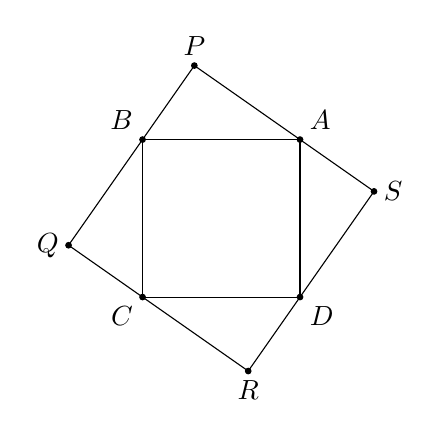
\begin{tikzpicture}
    \draw (-1,-1)--(-1,1)--(1,1)--(1,-1)--cycle;
    \filldraw (-1,-1) circle (1pt) node[anchor=north east] {$C$};
    \filldraw (-1,1) circle (1pt) node[anchor=south east] {$B$};
    \filldraw (1,1) circle (1pt) node[anchor=south west] {$A$};
    \filldraw (1,-1) circle (1pt) node[anchor=north west] {$D$};
    
    \draw (-0.342020143,1.93969262)--(1.93969262,0.342020143)--(0.342020143,-1.93969262)--(-1.93969262,-0.342020143)--cycle;
    \filldraw (-0.342020143,1.93969262) circle (1pt) node[anchor=south] {$P$};
    \filldraw (1.93969262,0.342020143) circle (1pt) node[anchor=west] {$S$};
    \filldraw (0.342020143,-1.93969262) circle (1pt) node[anchor=north] {$R$};
    \filldraw (-1.93969262,-0.342020143) circle (1pt) node[anchor=east] {$Q$};
    \end{tikzpicture}}
\end{addsol}
\end{solu}

\item (USAJMO 2020/4) Let $ABCD$ be a convex quadrilateral inscribed in a circle and satisfying $DA < AB = BC < CD$. Points $E$ and $F$ are chosen on sides $CD$ and $AB$ such that $BE \perp AC$ and $EF \parallel BC$. Prove that $FB = FD$.

\item (IMO 2006/1) Let $ABC$ be triangle with incenter $I$. A point $P$ in the interior of the triangle satisfies\[\angle PBA+\angle PCA = \angle PBC+\angle PCB.\]Show that $AP \geq AI$, and that equality holds if and only if $P=I$.

\end{enumerate}

\subsection{Challenges}

\begin{enumerate}

	\item (MAST Diagnostic 2020) Consider parallelogram $ABCD$ with $AB=7,$ $BC=6.$ Let the angle bisector of $\angle DAB$ intersect $BC$ at $X$ and $CD$ at $Y.$ Let the line through $X$ parallel to $BD$ intersect $AD$ at $Q.$ If $QY=6,$ find $\cos\angle DAB.$
	\begin{hint}
	\begin{addhint}
	{How would you find $BX$ and $DY?$}
	\end{addhint}
	\begin{addhint}
	{Remember that $QX$ and $DB$ are parallel. How does this help you find $QD?$}
	\end{addhint}
	\end{hint}
	\begin{solu}
	\begin{addsol}
	{Note that $\triangle ABX$ and $\triangle ADY$ are isosceles, so $BX=7$ and $DY=6.$ Now also note that $XQDB$ is a parallelogram, so $QD=BX=7.$ Now note $\angle QDY=\angle DAB,$ so it suffices to find $\cos\angle QDY.$
	
	Now note that $QY=DY=6$ and $QD=7.$ Thus dropping the altitude from $Y$ to $QD$ gives us $\cos \angle QDY=\frac{\frac{7}{2}}{6}=\frac{7}{12}.$}
	\end{addsol}
	\end{solu}

    \item (Memorial Day Mock AMC 10 2018/21) In the following diagram, $m\angle BAC=m\angle BFC=40^{\circ}$, $m\angle ABF=80^{\circ}$, and $m\angle FEB=2m\angle DBE=2m\angle FBE$. What is $m\angle ADB$?

    \begin{center}
    \begin{asy}
    size(4cm);
    draw((0,0)--(-14,0)--(2,8)--(0,0)--(-9,2.5)--(-5.5,0)--(-6,4)--cycle);
    draw((-5.5,0)--(2,8));
    label("A", (2,8), NE);
    label("B", (0,0), SE);
    label("C", (-5.5,0), S);
    label("D", (-14,0), SW);
    label("E", (-9,2.5), NNW);
    label("F", (-6,4), NNW);
    \end{asy}
    \end{center}
    
    \begin{hint}
    \begin{addhint}
    {Look for cyclic quadrilaterals.}
    \end{addhint}
    \begin{addhint}
    {Use Tangent/Secant to set up a system of equations.}
    \end{addhint}
    \end{hint}
    
    \item (FARML 2012/6) In triangle $ABC,$ $AB=7,$ $AC=8,$ and $BC=10.$ $D$ is on $AC$ and $E$ is on $BC$ such that $\angle AEC=\angle BED=\angle B+\angle C.$ Compute the length $AD.$
    \begin{hint}
    \begin{addhint}
    {Look for similar triangles.}
    \end{addhint}
    \begin{addhint}
    {Prove $\triangle ABC\sim \triangle EDC\sim \triangle EBA.$}
    \end{addhint}
    \end{hint}
    \begin{solu}
\begin{addsol}
{Angle chase to find $\triangle ABC\sim \triangle EDC\sim \triangle EBA.$ So $BE=7\cdot\frac{7}{10}=\frac{49}{10},$ implying $CE=10-\frac{49}{10}=\frac{51}{10},$ and $CD=\frac{10}{8}\cdot\frac{51}{10}=\frac{51}{8},$ implying $AD=8-\frac{51}{8}=\frac{13}{8}.$}
\end{addsol}
\end{solu}
    
    \item (ISL 1994/G1) $C$ and $D$ are points on a semicircle. The tangent at $C$ meets the extended diameter of the semicircle at $B$, and the tangent at $D$ meets it at $A$, so that $A$ and $B$ are on opposite sides of the center. The lines $AC$ and $BD$ meet at $E$. $F$ is the foot of the perpendicular from $E$ to $ AB$. Show that $EF$ bisects angle $CFD.$
    \begin{hint}
    \begin{addhint}
    {Where do $BC$ and $DA$ meet?}
    \end{addhint}
    \begin{addhint}
    {Draw in the center of the semicircle.}
    \end{addhint}
    \begin{addhint}
    {Look for similar triangles.}
    \end{addhint}
    \end{hint}
    \begin{solu}
    \begin{addsol}
    {The key observation is that $AD,BC,EF$ concur.
    
    Let $AD$ and $BC$ intersect at $P$ and let $Q$ be the foot of the altitude from $P$ to $AB.$ Also let the semicircle have center $O.$ Now note
    \[\triangle PAQ\sim \triangle OAD\]
    \[\triangle PBQ\sim \triangle OBC\]
    so $\frac{AQ}{QB}\cdot\frac{BC}{CP}\cdot\frac{PD}{DA}=1.$ Since $AC,BD,PQ$ concur, $Q$ is actually $F,$ and $AC,BD,PF$ concur.
    
    Now note
    \[\angle OCP=\angle ODP=\angle OFP=90^{\circ},\]
    so $OFCPD$ is cyclic. Thus
    \[\angle COP=\angle DOP\]
    \[\angle CFP=\angle DFP.\]}
    \end{addsol}
    \end{solu}
    
    \item Consider $\triangle ABC$ with $D$ on line $BC.$ Let the circumcenters of $\triangle ABD$ and $\triangle ACD$ be $M,N,$ respectively. Let the circumcircle of $\triangle MND$ intersect the circumcircle of $\triangle ACD$ again at $H\neq D.$ Prove that $A,M,H$ are collinear.
    \begin{hint}
    \begin{addhint}
    {Look for similar and congruent triangles.}
    \end{addhint}
    \begin{addhint}
    {What does $\triangle AMN\sim\triangle DMN\sim\triangle ABC$ tell you?}
    \end{addhint}
    \end{hint}
    
    \item (APMO 1999/3) Let $\Gamma_1$ and $\Gamma_2$ be two circles intersecting at $P$ and $Q$. The common tangent, closer to $P$, of $\Gamma_1$ and $\Gamma_2$ touches $\Gamma_1$ at $A$ and $\Gamma_2$ at $B$. The tangent of $\Gamma_1$ at $P$ meets $\Gamma_2$ at $C$, which is different from $P$, and the extension of $AP$ meets $BC$ at $R$.
Prove that the circumcircle of triangle $PQR$ is tangent to $BP$ and $BR$.
    \begin{hint}
    \begin{addhint}
    {Show that $BP=BR.$}
    \end{addhint}
    \begin{addhint}
    {$R$ seems somewhat pesky. Can you find other stuff $R$ is involved with?}
    \end{addhint}
    \begin{addhint}
    {Prove that $ABRQ$ is cyclic.}
    \end{addhint}
    \begin{addhint}
    {Reflect $P$ about the midpoint of $AB.$}
    \end{addhint}
    \end{hint}
    \begin{solu}
    \begin{addsol}
    {Note that
\[\angle BPR=\angle BAP+\angle ABP=\angle AQP+\angle PBQ=\angle AQB\]
and that
\[\angle BRP=\angle RPC+\angle RCP=180^{\circ}-\angle APC+\angle BCP=\angle AQP+\angle BQP=\angle AQB,\]
so $\angle BPR=\angle BRP.$

Now note
\[\angle AQB=\angle BAP+\angle ABP=180^{\circ}-\angle APB=\angle BPR=\angle BRP,\]
so $ABRQ$ is cyclic.

Now reflect $P$ about the midpoint of $AB$ to get $P'.$ Then note
\[\angle PQR=\angle P'QR=\angle P'AR=\angle P'AB+\angle BAR=\angle ABR+\angle BAP=\angle BPR,\]
so $BP$ is tangent to $(PQR),$ as desired.}
    \end{addsol}
    \end{solu}
    
    \item Let $K_1$ and $K_2$ be circles that intersect at two points $A$ and $B.$ The tangents to $K_1$ at $A$ and $B$ intersect at a point $P$ inside $K_2,$ and the line $BP$ intersects $K_2$ again at $C.$ The tangents to $K_2$ at $A$ and $C$ intersect at a point $Q,$ and the line $QA$ intersects $K_1$ again at $D.$

Prove that $QP$ is perpendicular to $PD$ if and only if the centre of $K_2$ lies on $K_1.$
\begin{hint}
\begin{addhint}
{Look for collinear points.}
\end{addhint}
\begin{addhint}
{There is a cyclic quadrilateral with $O_2$ on it.}
\end{addhint}
\end{hint}
\begin{solu}
\begin{addsol}
{Say the center of $K_1$ is $O_1$ and the center of $K_2$ is $O_2.$ Obviously $AO_2CQ$ is cyclic since $\angle QAO_2=\angle QCO_2=90^{\circ}.$ Now note $\angle QCP=180-\angle BAC,$ and $\angle PAB=\angle ABP=\angle ABC=\angle QAC,$ so $P$ also lies on this circle. Thus $\angle O_2PQ=90^{\circ}.$ Note
\[\angle ABO_2=\frac{180^{\circ}-\angle AO_2B}{2}=90^{\circ}-\angle ACB=90^{\circ}-\angle ACP=90^{\circ}-\angle AQP=90^{\circ}-\angle DQP,\]
and $\angle O_2DA=\angle O_2BA$ if and only if $O_2$ lies on $(ABD),$ or $K_1.$ Then $\angle O_2DA=\angle O_2BA$ implies that $\angle DPQ=90^{\circ},$ as desired.}
\end{addsol}
\end{solu}
    
    \item (IMO 2000/1) Two circles $G_1$ and $G_2$ intersect at two points $M$ and $N$. Let $AB$ be the line tangent to these circles at $A$ and $B$, respectively, so that $M$ lies closer to $AB$ than $N$. Let $CD$ be the line parallel to $AB$ and passing through the point $M$, with $C$ on $G_1$ and $D$ on $G_2$. Lines $AC$ and $BD$ meet at $E$; lines $AN$ and $CD$ meet at $P$; lines $BN$ and $CD$ meet at $Q$. Show that $EP=EQ$.
\begin{hint}
\begin{addhint}
{What is the foot of the perpendicular from $E$ to $PQ?$}
\end{addhint}
\begin{addhint}
{Let $MN$ intersect $AB$ at $O.$}
\end{addhint}
\end{hint}
\begin{solu}
\begin{addsol}
{Notice $\angle EAB=\angle ACM=\angle ANM=\angle BAM$ and $\angle EBA=\angle ABM,$ so $\triangle EAB\cong \triangle MAB,$ implying that $AB$ is the perpendicular bisector of $EM.$ So $\angle EMP=\angle EMQ=90^{\circ},$ and it suffices to show that $PM=MQ.$

Let $MN$ intersect $AB$ at $O.$ Note that $AO=BO,$ so $PM=MQ$ by similar triangles.}
\end{addsol}
\end{solu}

\end{enumerate}

\chapter{Power of a Point}

\chapterquote{You're a wizard, Harry.}{Harry Potter and the Philosopher's Stone}

There's only one theorem, so this will be a short chapter. The only prerequisites are angle chasing theorems in circles.

\section{Power of a Point}

The Power of a Point theorem helps us length chase in circles. The proof is a result of similar triangles, and its uses are numerous in lower-level competitions. If you already know this theorem, feel free to skip this section.

\begin{theo}[Power of a Point]
Let line $\ell_1$ intersect circle $\omega$ at $A,B$ line $\ell_2$ intersect $\omega$ at $C,D,$ and $\ell_1$ intersect $\ell_2$ at $P.$ Then $PA\cdot PB=PC\cdot PD.$
\end{theo}

\begin{pro}
There are two cases here: Either $P$ is inside of $\omega$ or outside of $\omega.$

If $P$ is inside of $\omega,$ then note that by Inscribed Angle, $\angle PAC=\angle PDB$ and $\angle=\angle PAB,$ so $\triangle PAC\sim \triangle PDB.$

If $P$ is outside of $\omega,$ then without loss of generality, let $PA\leq PB$ and $PC\leq PD.$ Then note $\angle PAC=180^{\circ}-\angle CAB=\angle PDB$ and $\angle PCA=180^{\circ}-\angle ACD=\angle PBD,$ so $\triangle PAC\sim\triangle PDB.$

To finish, note that the similarity implies $\frac{PA}{PC}=\frac{PD}{PB}$, or $PA\cdot PB=PC\cdot PB.$

\begin{center}
\begin{asy}
size(4cm);
//Generated By AsyPadv1.2
import olympiad;
import markers;
import math;
import graph;

//colored pens
pen c000000 = rgb("000000");
//dependency level 0
/* You can change the coordinates of these points of dependency level 0.
The drawing will retain the same relationships and qualities.
Please be aware that as a result of this some of the image may be clipped off. */
pair A = (4.72, 17.13); dot(A, c000000); label("$A$", A, dir(136.636577041617));
pair B = (4.38, 16.06); dot(B, c000000); label("$D$", B, dir(236.09372301155847));
pair C = (6.13, 15.99); dot(C, c000000); label("$B$", C, dir(319.3987053549977));
//dependency level 1
//Do not change anything below, unless you are experienced in Asymptote.
path ccA_B_C = circumcircle(A, B, C);
pair ccA_B_Ccenter = circumcenter(A, B, C); real ccA_B_Crad = circumradius(A, B, C); draw(ccA_B_C, c000000);
path segA_C = A--C; draw(segA_C, c000000);
//dependency level 2
pair D = relpoint(ccA_B_C, 0.1252472145174768); dot(D, c000000); label("$C$", D, dir(48.14541204060811));
//dependency level 3
path segB_D = B--D; draw(segB_D, c000000);
//dependency level 4
pair P = intersectionpoint(segA_C, segB_D); dot(P, c000000); label("$P$", P, dir(79.06275557490466));
\end{asy}
\begin{asy}
//Generated By AsyPadv1.2
import olympiad;
import markers;
import math;
import graph;
//change the unit size to fit your needs
size(4cm);
//colored pens
pen c000000 = rgb("000000");
//dependency level 0
/* You can change the coordinates of these points of dependency level 0.
The drawing will retain the same relationships and qualities.
Please be aware that as a result of this some of the image may be clipped off. */
pair A = (3.47, 17.85); dot(A, c000000); label("$A$", A, dir(126.02737338510292));
pair B = (2.88, 16.31); dot(B, c000000); label("$B$", B, dir(236.09372301155847));
pair C = (4.64, 16.25); dot(C, c000000); label("$C$", C, dir(319.3987053549977));
//dependency level 1
//Do not change anything below, unless you are experienced in Asymptote.
path ccA_B_C = circumcircle(A, B, C);
pair ccA_B_Ccenter = circumcenter(A, B, C); real ccA_B_Crad = circumradius(A, B, C); draw(ccA_B_C, c000000);
path lineB_A = (B-20.0*unit(A-B))--(A+20.0*unit(A-B)); 
//dependency level 2
pair D = relpoint(ccA_B_C, 0.21889966793444027); dot(D, c000000); label("$D$", D, dir(48.14541204060811));
//dependency level 3
path lineD_C = (D-20.0*unit(C-D))--(C+20.0*unit(C-D)); 
//dependency level 4
pair P = intersectionpoint(lineB_A, lineD_C); dot(P, c000000); label("$P$", P, dir(84.11889062937553));
//dependency level 5
path segP_B = P--B; draw(segP_B, c000000);
path segP_C = P--C; draw(segP_C, c000000);
\end{asy}

\textit{$P$ inside $\omega$ and $P$ outside $\omega.$}
\end{center}
\end{pro}

In the case of tangency, $A=B$ is the point of tangency. (You can think of a tangent line intersecting a circle twice at the same point.)

The Two Tangent Theorem is a corollary of Power of a Point. It states that the lengths of the two tangents from a point to a circle are equal.

\begin{fact}[Two Tangent Lemma]
Let the tangents from point $P$ to circle $\omega$ intersect $\omega$ at $A,B.$ Then $PA=PB.$
\begin{hint}
\begin{addhint}
{Use power of a point to relate $PA$ and $PB.$}
\end{addhint}
\end{hint}
\begin{solu}
\begin{addsol}
{Note that by Power of a Point, $PA^2=PB^2.$

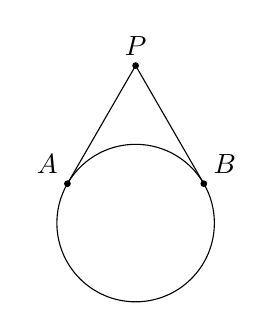
\begin{tikzpicture}
\draw (-0.8660254037844386,0.5)--(0,2)--(0.8660254037844386,0.5);
\draw (0,0) circle (1);
\filldraw (-0.8660254037844386,0.5) circle (1pt) node[anchor=south east] {$A$};
\filldraw (0.8660254037844386,0.5) circle (1pt) node[anchor=south west] {$B$};
\filldraw (0,2) circle (1pt) node[anchor=south] {$P$};
\end{tikzpicture}}
\end{addsol}
\end{solu}
\end{fact}

\section{Bisector Lemma}

This is a very powerful fact that kills a lot of earlier computational geometry problems involving circles.

\begin{fact}[Bisector Lemma]
Let $\omega_1$ and $\omega_2$ intersect at $X$ and $Y,$ and let $\ell$ be a line tangent to $\omega_1$ and $\omega_2.$ If $\ell$ intersects $\omega_1$ at $A$ and $\omega_2$ at $B,$ then $XY$ bisects $AB.$
\end{fact}

\begin{pro}
Let $XY$ intersect $AB$ at $P.$ Then by Power of a Point, $PX^2=PA\cdot PB=PY^2.$
\begin{center}
\begin{asy}
size(6cm);
real xmin = -4.5, xmax = 4, ymin = -3, ymax = 35;

draw(circle((-2,0), 2.23606797749979)); 
draw(circle((1,0), 2.8284271247461903)); 
draw((xmin, 0.20141850719855647*xmin + 2.68381204170681)--(xmax, 0.20141850719855647*xmax + 2.68381204170681)); /* line */
draw((-1,2.4823935345082537)--(-1,-2)); 

dot("$X$",(-1,2),dir(5));
dot("$Y$",(-1,-2),dir(55));
dot("$A$",(-2.4415184401122536,2.1920450422016526),dir(100)); 
dot("$B$",(0.44151844011225216,2.7727420268148544),dir(100)); 
dot("$P$",(-1,2.4823935345082537),dir(100)); 
clip((xmin,ymin)--(xmin,ymax)--(xmax,ymax)--(xmax,ymin)--cycle); 
\end{asy}
\end{center}
\end{pro}

\section{Summary}

\subsection{Theory}

\begin{enumerate}
\item Power of a Point
\begin{itemize}
\Item If lines $\ell_1,\ell_2$ through $P$ intersect circle $\omega$ at $A,B$ and $C,D,$ respectively, then $PA\cdot PB=PC\cdot PD.$

\Item This is a consequence of similar triangles.
\end{itemize}
\item Bisector Lemma
\begin{itemize}
\Item The common chord of two circles bisects the common external tangent.
\end{itemize}
\end{enumerate}

\subsection{Tips and Strategies}

\begin{enumerate}
\item If there are two circles and you're in doubt, use Bisector Lemma. (This even applies for some easier olympiad problems.)
\end{enumerate}

\pagebreak

\section{Exercises}

\subsection{Check-ins}

\begin{enumerate}
\item Let chords $AB$ and $CD$ in circle $\omega$ intersect at $P.$ If $AP=BP=4$ and $CP=2,$ find $DP.$

\begin{asy}
//Generated By AsyPadv1.2
import olympiad;
import markers;
import math;
import graph;
//change the unit size to fit your needs
size(3cm);
//colored pens
pen c000000 = rgb("000000");
//dependency level 0
/* You can change the coordinates of these points of dependency level 0.
The drawing will retain the same relationships and qualities.
Please be aware that as a result of this some of the image may be clipped off. */
pair A = (3.32, 17.11); dot(A, c000000); label("$A$", A, dir(207.8972710309471));
pair B = (5.05, 17.09); dot(B, c000000); label("$B$", B, dir(325.00797980144));
//dependency level 1
//Do not change anything below, unless you are experienced in Asymptote.
path pbA_B = ((A+B)/2-20.0*unit(((B-A).y, -(B-A).x)))--((A+B)/2+20.0*unit(((B-A).y, -(B-A).x))); 
path segA_B = A--B; draw(segA_B, c000000);
//dependency level 2
pair C = relpoint(pbA_B, 0.5134646278119219); dot(C, c000000); label("$C$", C, dir(274.31287501714553));
pair P = intersectionpoint(pbA_B, segA_B); dot(P, c000000); label("$P$", P, dir(50.95410743116071));
//dependency level 3
path ccA_C_B = circumcircle(A, C, B);
pair ccA_C_Bcenter = circumcenter(A, C, B); real ccA_C_Brad = circumradius(A, C, B); draw(ccA_C_B, c000000);
//dependency level 4
pair D = intersectionpoints(pbA_B, ccA_C_B)[0]; dot(D, c000000); label("$D$", D, dir(88.75312672365999));
//dependency level 5
path segD_C = D--C; draw(segD_C, c000000);
\end{asy}

\item Let the tangent through $A$ to circle $\omega$ intersect line $\ell$ that passes through $B,C$ on $\omega$ at $P.$ If $BP<CP,$ $AP=4,$ and $BC=6,$ find $BP.$

\begin{asy}
import olympiad;
import markers;
import math;
import graph;
//change the unit size to fit your needs
size(3cm);
//colored pens
pen c000000 = rgb("000000");
//dependency level 0
/* You can change the coordinates of these points of dependency level 0.
The drawing will retain the same relationships and qualities.
Please be aware that as a result of this some of the image may be clipped off. */
pair C = (4.51, 16.84); dot(C, c000000); label("$C$", C, dir(25.70995378080977));
pair D = (3.19, 16.32); 
pair P = (2.25, 18.25); dot(P, c000000); label("$P$", P, dir(91.48786752882734));
//dependency level 1
//Do not change anything below, unless you are experienced in Asymptote.
path circD_C = Circle(D, abs(D-C));
pair circD_Ccenter = D; real circD_Crad = abs(D - C); draw(circD_C, c000000);
path segP_C = P--C; draw(segP_C, c000000);
//dependency level 2
pair P_circD_C_tangent1 = tangent(P, circD_Ccenter, circD_Crad, 1);
path tl1P_circD_C = (P-20.0*unit(P_circD_C_tangent1-P))--(P_circD_C_tangent1+20.0*unit(P_circD_C_tangent1-P)); 
pair B = intersectionpoints(segP_C, circD_C)[0]; dot(B, c000000); label("$B$", B, dir(81.55446702351315));
//dependency level 3
pair A = tangent(P,circD_Ccenter, circD_Crad,1);
dot("$A$", A, dir(155.9863895131953));
//dependency level 4
path segP_A = P--A; draw(segP_A, c000000);
\end{asy}

\item Let line $\ell_1$ that passes through $A,B$ on circle $\omega$ intersect line $\ell_2$ that passes through $C,D$ on $\omega$ at $P.$ If $PA=6,$ $AB=12,$ and $PC=3,$ find $CD.$

\begin{asy}
//Generated By AsyPadv1.2
import olympiad;
import markers;
import math;
import graph;
//change the unit size to fit your needs
size(3cm);
//colored pens
pen c000000 = rgb("000000");
//dependency level 0
/* You can change the coordinates of these points of dependency level 0.
The drawing will retain the same relationships and qualities.
Please be aware that as a result of this some of the image may be clipped off. */
pair D = (4.25, 16.81); dot(D, c000000); label("$D$", D, dir(25.70995378080977));
pair O = (3.19, 16.32); 
pair P = (2.71, 17.84); dot(P, c000000); label("$P$", P, dir(91.48786752882734));
//dependency level 1
//Do not change anything below, unless you are experienced in Asymptote.
path circO_D = Circle(O, abs(O-D));
pair circO_Dcenter = O; real circO_Drad = abs(O - D); draw(circO_D, c000000);
path segP_D = P--D; draw(segP_D, c000000);
//dependency level 2
pair C = intersectionpoints(segP_D, circO_D)[0]; dot(C, c000000); label("$C$", C, dir(81.55446702351315));
pair B = relpoint(circO_D, -0.4892866639289171); dot(B, c000000); label("$B$", B, dir(315.0));
//dependency level 3
path segP_B = P--B; draw(segP_B, c000000);
//dependency level 4
pair A = intersectionpoints(segP_B, circO_D)[0]; dot(A, c000000); label("$A$", A, dir(315.0));
\end{asy}

\item Let $\triangle ABC$ have a right angle at $C$ and let $P$ be the foot of the altitude from $C$ to $AB.$ If the foot of the altitude from $P$ to $AC$ is $X$ and the foot from $P$ to $BC$ is $Y,$ then prove that $AXYB$ is cyclic.
\end{enumerate}

\subsection{Problems}

\begin{enumerate}
\item Let $PA$ and $PB$ be tangents to circle $\omega,$ and let line $\ell$ through $P$ intersect $\omega$ at $X$ and $C$ and $AB$ at $Y.$ If $PA=4$, $PC=8,$ $AY=1$, and $XY=1,$ find the area of $\triangle PAB.$

\begin{asy}
//Generated By AsyPadv1.2
import olympiad;
import markers;
import math;
import graph;
//change the unit size to fit your needs
size(6cm);
//colored pens
pen c000000 = rgb("000000");
//dependency level 0
/* You can change the coordinates of these points of dependency level 0.
The drawing will retain the same relationships and qualities.
Please be aware that as a result of this some of the image may be clipped off. */
pair B = (3.88, 17.20); dot(B, c000000); label("$B$", B, dir(51.60483549675433));
pair O = (3.19, 16.32); 
//dependency level 1
//Do not change anything below, unless you are experienced in Asymptote.
path circO_B = Circle(O, abs(O-B));
pair circO_Bcenter = O; real circO_Brad = abs(O - B); draw(circO_B, c000000);
path segO_B = O--B; 
//dependency level 2
pair C = relpoint(circO_B, -0.3326246702692839); dot(C, c000000); label("$C$", C, dir(253.50839790887915));
pair A = relpoint(circO_B, -0.6270403362062634); dot(A, c000000); label("$A$", A, dir(120.96189753921033));
path perB_segO_B = (B-20.0*(dir(segO_B).y, -dir(segO_B).x))--(B+20.0*(dir(segO_B).y, -dir(segO_B).x)); 
//dependency level 3
path segA_O = A--O; 
path segA_B = A--B; draw(segA_B, c000000);
//dependency level 4
path perA_segA_O = (A-20.0*(dir(segA_O).y, -dir(segA_O).x))--(A+20.0*(dir(segA_O).y, -dir(segA_O).x)); 
//dependency level 5
pair P = intersectionpoint(perA_segA_O, perB_segO_B); dot(P, c000000); label("$P$", P, dir(88.28051995968144));
//dependency level 6
path segP_C = P--C; draw(segP_C, c000000);
path segP_A = P--A; draw(segP_A, c000000);
path segP_B = P--B; draw(segP_B, c000000);
//dependency level 7
pair X = intersectionpoints(segP_C, circO_B)[0]; dot(X, c000000); label("$X$", X, dir(129.2296640975739));
pair Y = intersectionpoint(segA_B, segP_C); dot(Y, c000000); label("$Y$", Y, dir(133.61835402638553));
//clip the drawing view
clip((0.0, 13.0)--(0.0, 20.0)--(10.0, 20.0)--(10.0, 13.0)--cycle);
\end{asy}


\item Consider two externally tangent circles $\omega_1,\omega_2.$ Let them have common external tangents $AC,BD$ such that $A,B$ are on $\omega_1$ and $C,D$ are on $\omega_2.$ Let $AC$ intersect $BD$ at $P,$ and let the common internal tangent intersect $AC$ and $BD$ at $X$ and $Y$. If $\frac{[PCD]}{[PAB]}=\frac{1}{25},$ find $\frac{[PCD]}{[PXY]}.$

\item (Mandelbrot 2012) Let $A$ and $B$ be points on the lines $y=3$ and $y=12,$ respectively. There are two circles passing through $A$ and $B$ that are also tangent to the $x$ axis, say at $P$ and $Q.$ Suppose that $PQ=2012.$ Find $AB.$

\item (Parody) Consider a coordinate plane with two circles tangent to the $x$ axis at $X,Y,$ respectively. If the circles intersect at $P,Q,$ and $XY=8,$ is it possible for $P$ to lie on $y=3$ and $Q$ to lie on $y=12?$

\item (e-dchen Mock MATHCOUNTS) Consider chord $AB$ of circle $\omega$ centered at $O.$ Let $P$ be a point on segment $AB$ such that $AP=2$ and $BP=8$. If $\angle APO=150^{\circ},$ what is the area of $\omega?$
\end{enumerate}

\section{Challenges}

\begin{enumerate}
	\item (Geometry Bee 2019) Circles $O_1$ and $O_2$ are constructed with $O_1$ having radius of $2,$ $O_2$ having radius of $4,$ and $O_2$ passing through the point $O_1.$ Lines $\ell_1$ and $\ell_2$ are drawn so they are tangent to both $O_1$ and $O_2.$ Let $O_1$ and $O_2$ intersect at points $P$ and $Q.$ Segment $\overline{EF}$ is drawn through $P$ and $Q$ such that $E$ lies on $\ell_1$ and $F$ lies on $\ell_2.$ What is the length of $\overline{EF}?$
	
\item (AMC 10B 2013/23) In triangle $ABC$, $AB=13$, $BC=14$, and $CA=15$. Distinct points $D$, $E$, and $F$ lie on segments $\overline{BC}$, $\overline{CA}$, and $\overline{DE}$, respectively, such that $\overline{AD}\perp\overline{BC}$, $\overline{DE}\perp\overline{AC}$, and $\overline{AF}\perp\overline{BF}$. The length of segment $\overline{DF}$ can be written as $\frac{m}{n}$, where $m$ and $n$ are relatively prime positive integers. What is $m+n$?
\begin{solu}
\begin{addsol}
{Let the circle with diameter $AB$ be $\omega.$ Note $\omega$ intersects $DE$ at $D,F$ and $AC$ at $H$ where $H$ is the foot of the altitude from $B$ to $AC.$

Now note $EF\cdot ED=EH\cdot EA,$ or $EF\cdot \frac{36}{5}=3\cdot \frac{48}{5}.$ So $EF=4$ and $DF=\frac{16}{5},$ so the answer is $21.$}
\end{addsol}
\end{solu}
\end{enumerate}

\chapter{Lengths and Areas in Triangles}

\chapterquote{Again, you can’t connect the dots looking forward; you can only connect them looking backward. So you have to trust that the dots will somehow connect in your future. You have to trust in something — your gut, destiny, life, karma, whatever. This approach has never let me down, and it has made all the difference in my life.}{Steve Jobs}

\section{Lengths}
There are a couple of important lengths in a triangle. These are the lengths of cevians, the inradius/exradius, and the circumradius.

\subsection{Law of Cosines and Stewart's}
We discuss how to find the third side of a triangle given two sides and an included angle, and use this to find a general formula for the length of a cevian.

\begin{theo}[Law of Cosines]
Given $\triangle ABC,$ $a^2+b^2-2ab\cos C=c^2.$
\end{theo}

\begin{pro}
Let the foot of the altitude from $A$ to $BC$ be $H.$ Then note that $A=b\sin C,$ $CH=b\cos C,$ and $BH=|a-b\cos C|.$ (The absolute value is because $\angle B$ can either be acute or obtuse.) Then note by the Pythagorean Theorem, $(b\sin C)^2+(a-b\cos C)^2=a^2+b^2-2ab\cos C=c^2.$
\begin{center}
    \begin{asy}
    size(4cm);
    dot((-3,0));
    dot((1,0));
    dot((0,3));
    dot((0,0));
    draw((-3,0)--(1,0)--(0,3)--cycle);
    draw((0,3)--(0,0));
    
    label("$C$",(-3,0),SW);
    label("$B$",(1,0),SE);
    label("$A$",(0,3),N);
    label("$H$",(0,0),S);
    \end{asy}
\end{center}
\end{pro}

\begin{theo}[Stewart's Theorem]
Consider $\triangle ABC$ with cevian $AD,$ and denote $BD=m,$ $CD=n,$ and $AD=d.$ Then $man+dad=bmb+cnc.$
\end{theo}

\begin{pro}
We use the Law of Cosines. Note that
\[\cos \angle ADB=\frac{d^2+m^2-c^2}{2dm}=-\frac{d^2+n^2-b^2}{2dn}=-\cos \angle ADC.\]
Multiplying both sides by $2dmn$ yields
\[c^2n-d^2n-m^2n=-bm^2+d^2m+mn^2\]
\[b^2m+c^2n=mn(m+n)+d^2(m+n)\]
\[bmb+cnc=man+dad.\]
\begin{center}
    \begin{asy}
    size(4cm);
    dot((-3,0));
    dot((1,0));
    dot((0,3));
    draw((-3,0)--(1,0)--(0,3)--cycle);
    draw((0,3)--(-1,0));
    
    label("$C$",(-3,0),SW);
    label("$B$",(1,0),SE);
    label("$A$",(0,3),N);
    label("$D$",(-1,0),S);
    \end{asy}
\end{center}
\end{pro}

Here are two corollaries that will save you a lot of time in computational contests.

\begin{fact}[Length of Angle Bisector]
In $\triangle ABC$ with angle bisector $AD,$ denote $BD=x$ and $CD=y.$ Then
\[AD=\sqrt{bc-xy}.\]
\end{fact}

\begin{fact}[Length of Median]
In $\triangle ABC$ with median $AD,$
\[AD=\frac{\sqrt{2b^2+2c^2-a^2}}{2}.\]
\end{fact}

\subsection{Law of Sines and the Circumradius}
The Law of Sines is a good way to length chase with a lot of angles.

\begin{theo}[Law of Sines]
In $\triangle ABC$ with circumradius $R,$
\[\frac{a}{\sin A}=\frac{b}{\sin B}=\frac{c}{\sin C}=2R.\]
\end{theo}

\begin{pro}
We only need to prove that $\frac{a}{\sin A}=2R,$ and the rest will follow.

Let the line through $B$ perpendicular to $BC$ intersect $(ABC)$ again at $A'.$ Then note that $A'C=2R$ by Thale's. By the Inscribed Angle Theorem, $\sin \angle CA'B=\sin A,$ so $\frac{a}{\sin A}=\frac{a}{\sin \angle CA'B}=\frac{a}{\frac{a}{2R}}=2R.$
\begin{center}
    \begin{asy}
    import olympiad;
size(4cm);
pair A=(-1,5), B=(-4,-1), C=(4,-1), X, O;
O = circumcenter(A,B,C);
X = (2O-C);

draw(C--A--B--C);
draw(C--X--B);
draw(circumcircle(A,B,C));

label("$A$",A,(-1,1));label("$B$",B,(-1,-1));label("$C$",C,(1,-1));label("$A'$",X,(-1,1));label("$O$",O,(1,1));

dot(A^^B^^C^^X^^O);
    \end{asy}
\end{center}
\end{pro}

Other texts will call this the Extended Law of Sines. But the Extended Law of Sines has a better proof than the "normal" Law of Sines, and redundancy is bad.

The Law of Sines gives us the Angle Bisector Theorem.

\begin{theo}[Angle Bisector Theorem]
Let $D$ be the point on $BC$ such that $\angle BAD=\angle DAC.$ Then $\frac{AB}{BD}=\frac{AC}{CD}.$
\end{theo}

\begin{pro}
By the Law of Sines, $\frac{\sin\angle ADB}{\sin\angle BAD}=\frac{AB}{BD}$ and $\frac{\sin\angle ADC}{\sin\angle CAD}=\frac{AC}{CD}.$ But note that $\angle BAD=\angle ADC$ and $\angle BAD+\angle CAD=180^{\circ},$ so $\frac{AB}{BD}=\frac{AC}{CD}.$
\begin{center}
    \begin{asy}
    import markers;
import olympiad;
size(4cm);
real a,b,c,d;
pair A=(1,9), B=(-11,0), C=(4,0), D; b = abs(C-A); c = abs(B-A); D = (b*B+c*C)/(b+c);
draw(A--B--C--A--D);
label("$A$",A,(1,1));label("$B$",B,(-1,-1));label("$C$",C,(1,-1));label("$D$",D,(0,-1)); dot(A^^B^^C^^D);
markangle(radius=15,n=1,B,A,D,marker(markinterval(stickframe(n=1,2mm),true)));
markangle(radius=15,n=1,D,A,C,marker(markinterval(stickframe(n=1,2mm),true)));
\end{asy}
\end{center}
\end{pro}

In fact, the Angle Bisector Theorem can be generalized in what is known as the ratio lemma.

\begin{theo}[Ratio Lemma]
Consider $\triangle ABC$ with point $P$ on $BC.$ Then $\frac{BP}{CP}=\frac{c\sin \angle BAP}{b\sin \angle CAP}.$
\end{theo}

The proof is pretty much identical to the proof for Angle Bisector Theorem.

\begin{pro}
By the Law of Sines, $BP=\frac{c\sin\angle BAP}{\sin\angle APB}$ and $CP=\frac{b\sin\angle CAP}{\sin\angle APC}.$ Since $\sin\angle APB=\sin\angle APC,$
\[\frac{BP}{CP}=\frac{c\sin \angle BAP}{b\sin \angle CAP}.\]
\end{pro}

Note that this remains true even if $P$ is on the \textit{extension} of $BC.$

\subsection{The Incircle, Excircle, and Tangent Chasing}
We provide formulas for the inradius, exradii, and take a look at some uses of the Two Tangent Theorem. Recall that the Two Tangent Theorem states that if the tangents from $P$ to $\omega$ intersect $\omega$ at $A,B,$ then $PA=PB.$

\begin{theo}[$rs$]
In $\triangle ABC$ with inradius $r,$
\[[ABC]=rs.\]
\end{theo}

\begin{pro}
Note that $[ABC]=r\cdot\frac{a+b+c}{2}=rs.$

\begin{center}
\begin{asy}
import olympiad;
size(4cm);
pair A = dir(110);
	pair B = dir(210);
	pair C = dir(330);
	pair I = incenter(A, B, C);
	draw(A--B--C--cycle);
	draw(A--I--B);
	draw(I--C);
	draw(circle(I,length(I-foot(I,B,C))));
	dot("$A$", A, dir(A));
	dot("$B$", B, dir(190));
	dot("$C$", C, dir(-10));
	dot("$I$", I, dir(270));
\end{asy}
\end{center}
\end{pro}

A useful fact of the incircle is that the length of the tangents from $A$ is $s-a.$ Similar results hold for the $B,C$ tangents to the incircle.

\begin{fact}[Tangents to Incircle]
Let the incircle of $\triangle ABC$ be tangent to $BC,CA,AB$ at $D,E,F.$ Then
\[AE=AF=s-a\]
\[BF=BD=s-b\]
\[CD=CE=s-c.\]
\end{fact}

\begin{pro}
Note that by the Two Tangent Theorem, $AE=AF=x,$ $BF=BD=y,$ and $CD=CE=z.$ Also note that
\[BD+CD=y+z=a\]
\[CE+EA=z+x=b\]
\[AF+FB=x+y=c.\]
Adding these equations gives $2x+2y+2z=a+b+c=2s,$ implying $x+y+z=s.$ Thus
\[x=AE=AF=s-a\]
\[y=BF=BD=s-b\]
\[z=CD=CE=s-c,\]
as desired.
\begin{center}
\begin{asy}
import olympiad;
size(4cm);
pair A = dir(110);
	pair B = dir(210);
	pair C = dir(330);
	pair I = incenter(A, B, C);
    pair D,E,F;
    D=foot(I,B,C);
    E=foot(I,C,A);
    F=foot(I,A,B);
	draw(A--B--C--cycle);
	draw(circle(I,length(I-foot(I,B,C))));
	dot("$A$", A, dir(A));
	dot("$B$", B, dir(190));
	dot("$C$", C, dir(-10));
    dot("$D$", D, dir(-90));
    dot("$E$", E, dir(40));
    dot("$F$", F, dir(155));
\end{asy}
\end{center}
\end{pro}

\begin{theo}[$r_a(s-a)$]
In $\triangle ABC$ with $A$ exradius $r_a,$
\[[ABC]=r_a(s-a).\]
\end{theo}

\begin{pro}
Let $AB,AC$ be tangent to the $A$ excircle at $P,Q,$ respectively, and let $BC$ be tangent to the $A$ excircle at $D.$ Then note that by the Two Tangent Theorem, $PB=BD$ and $DC=CQ.$ Thus $[ABC]=[API_A]+[AQI_A]-2[BI_AC]=r_a\cdot \frac{s+s-2a}{2}=r_a(s-a).$
\end{pro}
\begin{center}
    \begin{asy}
    import olympiad;
    pair excenter(pair X, pair Y, pair Z){
pair A, C;
A=X+expi((angle(X-Y)+angle(Z-X))/2);
C=Z+expi((angle(Z-Y)+angle(X-Z))/2);
return extension(A,X,C,Z);
}
    size(4cm);
    pair A = dir(110);
	pair B = dir(210);
	pair C = dir(330);
	real a,b,c;
    a=abs(B-C); b = abs(C-A); c = abs(B-A);
	pair I = incenter(A, B, C);
	pair exa=excenter(C,A,B);
	draw(A--B--C--cycle);
	pair L = dir(270);
	pair I_A = 2*L-I;
	pair D=foot(I_A,B,C);
    pair P=foot(I_A,A,B);
    pair Q=foot(I_A,A,C);
    draw(B--P);
	draw(C--Q);
    dot("$A$", A, dir(A));
	dot("$B$", B, dir(190));
	dot("$C$", C, dir(0));
	dot("$I_A$", I_A, dir(I_A));
	dot("$D$",D,dir(270));
	draw(circle(exa,length(exa-foot(exa,B,C))));
    dot("$P$",P,dir(190));
    dot("$Q$",Q,dir(350));
    draw(P--I_A--Q,dotted);
    draw(A--I_A,dotted);
    \end{asy}
\end{center}

The proof also implies the following corollary.

\begin{fact}[Tangents to Excircle]
Let the $A$ excircle of $\triangle ABC$ be tangent to $BC$ at $D$. Then $BD=s-c$ and $CD=s-b.$

Analogous equations hold for the $B$ and $C$ excircles.
\end{fact}

\begin{pro}
Let the $A$ excircle be tangent to line $AB$ at $P$ and line $AC$ at $Q.$ Note that $AP=AB+BP=c+BD$ and $AQ=AC+CQ=b+CD$ by the Two Tangent Theorem. Applying the Two Tangent Theorem again gives $AP=AQ,$ or $c+BD=b+CD.$ Also note that $AP+AQ=b+c+BD+DC=2s,$ so $AP=AQ=s$ and $s=c+BD=b+CD.$ Thus $BD=s-c$ and $CD=s-b.$
\begin{center}
\begin{asy}
import olympiad;
    pair excenter(pair X, pair Y, pair Z){
pair A, C;
A=X+expi((angle(X-Y)+angle(Z-X))/2);
C=Z+expi((angle(Z-Y)+angle(X-Z))/2);
return extension(A,X,C,Z);
}
    size(4cm);
    pair A = dir(110);
	pair B = dir(210);
	pair C = dir(330);
	real a,b,c;
    a=abs(B-C); b = abs(C-A); c = abs(B-A);
	pair I = incenter(A, B, C);
	pair exa=excenter(C,A,B);
	draw(A--B--C--cycle);
	pair L = dir(270);
	pair I_A = 2*L-I;
	pair D=foot(I_A,B,C);
    pair P=foot(I_A,A,B);
    pair Q=foot(I_A,A,C);
    draw(B--P);
	draw(C--Q);
    dot("$A$", A, dir(A));
	dot("$B$", B, dir(190));
	dot("$C$", C, dir(0));
	dot("$D$",D,dir(270));
	draw(circle(exa,length(exa-foot(exa,B,C))));
    dot("$P$",P,dir(190));
    dot("$Q$",Q,dir(350));
\end{asy}
\end{center}
\end{pro}

Keep these area and length conditions in mind when you see incircles and excircles.

\subsection{Concurrency with Cevians}
We discuss Ceva's Theorem, Menelaus Theorem, and mass points, three ways to look at concurrent cevians. Very rarely do problems involving concurrency with cevians appear on higher level contests, but they're fairly common in the AMC 8 and MATHCOUNTS. This is also a good tool to have for when you need it.

\begin{theo}[Ceva's Theorem]
In $\triangle ABC$ with cevians $AD,BE,CF,$ they concur if and only if $\frac{AF}{FB}\cdot\frac{BD}{DC}\cdot\frac{CE}{EA}=1.$
\end{theo}

\begin{pro}
Let the point of concurrency be $P.$ Note that $\frac{[ABD]}{[ADC]}=\frac{[PBD]}{[PDC]}=\frac{BD}{DC},$ so $\frac{[BPA]}{[APC]}=\frac{BD}{DC}.$ Thus,
\[\frac{CE}{EA}\cdot\frac{AF}{FB}\cdot\frac{BD}{DC}=\frac{[CPB]}{[BPA]}\cdot\frac{[APC]}{[CPB]}\cdot\frac{[BPA]}{[APC]}=1.\]
\begin{center}
    \begin{asy}
    size(4cm);
pen rvwvcq = rgb(0.08235294117647059,0.396078431372549,0.7529411764705882); pen dtsfsf = rgb(0.8274509803921568,0.1843137254901961,0.1843137254901961); 

draw((0,0)--(1.62,0), rvwvcq); 
draw((1.62,0)--(4,0), dtsfsf); 
draw((2.9622788457580373,1.7295352570699383)--(4,0), rvwvcq); 
draw((2.9622788457580373,1.7295352570699383)--(1.84,3.6), dtsfsf); 
draw((1.84,3.6)--(0.7107411428354, 1.390580496852), rvwvcq); 
draw((0.7107411428354, 1.390580496852)--(0,0), dtsfsf); 

draw((1.84,3.6)--(1.62,0));
draw((0,0)--(2.9622788457580373,1.7295352570699383));
draw((4,0)--(0.7107411428354, 1.390580496852));

dot((1.679940099448, 0.9808379909682));
label("$P$",(1.679940099448, 0.9808379909682),N+0.5E);

dot((1.84,3.6)); 
label("$A$", (1.84,3.6), N); 
dot((0,0)); 
label("$B$", (0,0), SW); 
dot((4,0)); 
label("$C$", (4,0), SE); 
dot((1.62,0)); 
label("$D$", (1.62, 0), S); 
dot((2.9622788457580373,1.7295352570699383)); 
label("$E$", (2.9622788457580373,1.7295352570699383), NE); 
dot((0.7107411428354, 1.390580496852)); 
label("$F$", (0.7107411428354, 1.390580496852), NW); 
    \end{asy}
\end{center}
\end{pro}

A good way to remember what goes in the numerator and denominator is by looking at the colors and thinking about them alternating.

We present an example of what not to do.

\begin{exam}[Order Mixed Up]
Consider $\triangle ABC$ with $D,E,F$ on $BC,CA,AB$ respectively, such that $BD=4,$ $DC=6,$ $AE=6,$ $EC=4,$ and $AF=BF=5.$ Are $AD,$ $BE,$ and $CF$ concurrent?
\end{exam}

\begin{sol}[(Bogus)]
Yes. Note that $\frac{4}{6}\cdot\frac{6}{4}\cdot\frac{5}{5}=1.$
\begin{center}
\begin{asy}
size(4cm);
pen rvwvcq = rgb(0.08235294117647059,0.396078431372549,0.7529411764705882); pen dtsfsf = rgb(0.8274509803921568,0.1843137254901961,0.1843137254901961); 

draw((0,0)--(1.62,0), rvwvcq); 
draw((1.62,0)--(4,0), dtsfsf); 
draw((2.9622788457580373,1.7295352570699383)--(4,0), dtsfsf); 
draw((2.9622788457580373,1.7295352570699383)--(1.84,3.6), rvwvcq); 
draw((1.84,3.6)--(0.92,1.8), rvwvcq); 
draw((0.92,1.8)--(0,0), dtsfsf); 

dot((1.84,3.6)); 
label("$A$", (1.84,3.6), N); 
dot((0,0)); 
label("$B$", (0,0), SW); 
dot((4,0)); 
label("$C$", (4,0), SE); 
dot((1.62,0)); 
label("$D$", (1.62, 0), S); 
dot((2.9622788457580373,1.7295352570699383)); 
label("$E$", (2.9622788457580373,1.7295352570699383), NE); 
dot((0.92,1.8)); 
label("$F$", (0.92,1.8), NW); 
\end{asy}
\end{center}
\end{sol}

This is not right, as the order of the lengths is messed up (intentionally) in the problem statement. (Also note the colors are messed up.) We now present the correct solution.

\begin{sol}[(Correct)]
No. Note that $\frac{BD}{DC}\cdot\frac{CE}{EA}\cdot\frac{AF}{FB}=\frac{4}{6}\cdot\frac{4}{6}\cdot\frac{5}{5}=\frac{4}{9},$ which is not $1.$
\begin{center}
\begin{asy}
size(4cm);
pen rvwvcq = rgb(0.08235294117647059,0.396078431372549,0.7529411764705882); pen dtsfsf = rgb(0.8274509803921568,0.1843137254901961,0.1843137254901961); 

draw((0,0)--(1.62,0), rvwvcq); 
draw((1.62,0)--(4,0), dtsfsf); 
draw((2.9622788457580373,1.7295352570699383)--(4,0), rvwvcq); 
draw((2.9622788457580373,1.7295352570699383)--(1.84,3.6), dtsfsf); 
draw((1.84,3.6)--(0.92,1.8), rvwvcq); 
draw((0.92,1.8)--(0,0), dtsfsf); 

dot((1.84,3.6)); 
label("$A$", (1.84,3.6), N); 
dot((0,0)); 
label("$B$", (0,0), SW); 
dot((4,0)); 
label("$C$", (4,0), SE); 
dot((1.62,0)); 
label("$D$", (1.62, 0), S); 
dot((2.9622788457580373,1.7295352570699383)); 
label("$E$", (2.9622788457580373,1.7295352570699383), NE); 
dot((0.92,1.8)); 
label("$F$", (0.92,1.8), NW); 
\end{asy}
\end{center}
\end{sol}

There is also a trigonometric version of this theorem. Its proof is left as an exercise for the more experienced reader If you are encountering this for the first time, following the hints as a walkthrough is recommended.
\begin{theo}[Trigonometric Ceva]
Let $D,$ $E,$ and $F$ be points on sides $BC,$ $CA,$ and $AB$ of $\triangle ABC.$ Then $AD,$ $BE,$ and $CF$ concur if and only if
\[\frac{\sin\angle CAD}{\sin\angle DAB}\cdot \frac{\sin\angle ABE}{\sin\angle EBC}\cdot \frac{\sin\angle BCF}{\sin\angle FCE}=1.\]
\begin{hint}
\begin{addhint}
{How can we relate lengths with angles?}
\end{addhint}
\begin{addhint}
{We can use the Law of Sines to relate lengths with angles.}
\end{addhint}
\begin{addhint}
{The Ratio Lemma will help you explicitly solve it.}
\end{addhint}
\begin{addhint}
{Find $\frac{\sin CAD}{\sin DAB}.$}
\end{addhint}
\begin{addhint}
{By the Law of Sines, $\frac{AB}{\sin \angle ADB}=\frac{BD}{\sin DAB}$ and $\frac{AC}{\sin \angle ADC}=\frac{DC}{\sin \angle CAD}.$}
\end{addhint}
\begin{addhint}
{This implies $\frac{AB}{BD \sin \angle ADB}=\frac{AC}{DC\sin \angle CAD},$ or $\frac{AB}{CA}=\frac{BD\sin \angle ADB}{DC\sin \angle CAD}.$}
\end{addhint}
\begin{addhint}
{Multiply $\frac{AB}{CA}=\frac{BD\sin \angle ADB}{DC\sin \angle CAD}$ with symmetric expressions and finish with Ceva.}
\end{addhint}
\end{hint}
\end{theo}

Here is a harder example that relies on the trigonometric form of Ceva.

\begin{exam}[Swiss Math Olympiad 2008/8]
Let $ABCDEF$ be a convex hexagon inscribed in a circle. Prove that the diagonals $AD, BE$ and $CF$ intersect at one point if and only if \[\frac{AB}{BC} \cdot \frac{CD}{DE}\cdot \frac{EF}{FA}=1.\]
\end{exam}

\begin{sol}
Using Ceva's on $\triangle ACE,$ gives us that $AD,$ $BE,$ and $CF$ concur if and only if
\[\frac{\sin\angle AEB}{\sin\angle BEC}\cdot \frac{\sin\angle CAD}{\sin\angle DAE}\cdot \frac{\sin\angle ECF}{\sin\angle FCA}=1.\]
But note that by the Law of Sines,
\[\frac{\sin\angle AEB}{\sin\angle BEC}=\frac{\frac{AB}{2R}}{\frac{BC}{2R}}=\frac{AB}{BC},\]
where $R$ is the circumradius of $(ABCDEF),$ so this is equivalent to
\[\frac{AB}{BC}\cdot \frac{CD}{DE}\cdot \frac{EF}{FA} =1.\]
\end{sol}

\begin{theo}[Menelaus]
Consider $\triangle ABC$ with $D,E,F$ on lines $BC,CA,AB,$ respectively. Then $D,E,F$ are collinear if $\frac{DB}{BF}\cdot\frac{FA}{AE}\cdot\frac{EC}{CD}=1.$
\end{theo}

This looks very similar to Ceva - in fact, the letters just switched. Instead of the line segments cycling through $D,E,F,$ they now cycle through $A,B,C.$

\begin{pro}
Draw a line through $A$ parallel to $DE$ and let it intersect $BC$ at $P.$ Then note that $\triangle ABP\sim\triangle FBD$ and $\triangle ECD\sim \triangle ACP,$ so
\[\frac{AF}{FB}=\frac{PD}{DB}\]
\[\frac{EC}{EA}=\frac{DC}{DP}\]
Multiplying the two together yields
\[\frac{AF}{FB}\cdot\frac{BD}{DC}=\frac{EA}{CE},\]
which implies that
\[\frac{AF}{FB}\cdot\frac{BD}{DC}\cdot\frac{CE}{EA}=1,\]
as desired.
\begin{center}
\begin{asy}
import olympiad;
size(4cm);
    pair A=(7,6), B=(0,0), C=(10,0), P=(4,0), Q=(6,8), R, K=(5.5,0);
    draw(A--K, dashed);
draw((0,0)--(10,0)--(7,6)--(0,0));
draw((7,6)--(6,8)--(4,0));
R=intersectionpoint(A--B,Q--P);
dot(A^^B^^C^^P^^Q^^R^^K);
label("A",A,(1,1));label("B",B,(-1,0));label("C",C,(1,0));label("D",P,(0,-1));label("E",Q,(1,0));label("F",R,(-1,1));
label("P",K,(0,-1));
\end{asy}
\end{center}
\end{pro}

The converse states that $\frac{DB}{BF}\cdot\frac{FA}{AE}\cdot\frac{EC}{CD}=-1,$ \textit{where all lengths are directed.} (The directed lengths are necessary. In the original theorem, fixing $D,E$ leaves two possible locations for $F,$ only one of which actually lies on $DE.$)

\begin{theo}[Mass Points]
Consider segment $XY$ with $P$ on $XY.$ Then assign \textit{masses} $\diamond X,\diamond Y$ to points $X,Y$ such that $\frac{XP}{YP}=\frac{\diamond Y}{\diamond X}.$

\begin{center}
    \begin{asy}
    size(4cm);
    draw((0,0)--(3,0));
    dot("$X$",(0,0),S);
    dot("$P$",(1,0),S);
    dot("$Y$",(3,0),S);
    \end{asy}
\end{center}

Now consider cevians $AD,BE,CF$ of $\triangle ABC$ that concur at some point $P.$ Then $\frac{AP}{PD}=\frac{\diamond B+\diamond C}{\diamond A}.$

This means that for $P$ on $XY,$ we can define $\diamond P=\diamond X+\diamond Y.$

\begin{center}
    \begin{asy}
    size(4cm);
draw((0,0)--(1.62,0)); 
draw((1.62,0)--(4,0)); 
draw((2.9622788457580373,1.7295352570699383)--(4,0)); 
draw((2.9622788457580373,1.7295352570699383)--(1.84,3.6)); 
draw((1.84,3.6)--(0.7107411428354, 1.390580496852)); 
draw((0.7107411428354, 1.390580496852)--(0,0)); 

draw((1.84,3.6)--(1.62,0));
draw((0,0)--(2.9622788457580373,1.7295352570699383));
draw((4,0)--(0.7107411428354, 1.390580496852));

dot((1.679940099448, 0.9808379909682));
label("$P$",(1.679940099448, 0.9808379909682),N+0.5E);

dot((1.84,3.6)); 
label("$A$", (1.84,3.6), N); 
dot((0,0)); 
label("$B$", (0,0), SW); 
dot((4,0)); 
label("$C$", (4,0), SE); 
dot((1.62,0)); 
label("$D$", (1.62, 0), S); 
dot((2.9622788457580373,1.7295352570699383)); 
label("$E$", (2.9622788457580373,1.7295352570699383), NE); 
dot((0.7107411428354, 1.390580496852)); 
label("$F$", (0.7107411428354, 1.390580496852), NW); 
    \end{asy}
\end{center}
\end{theo}

This is a direct application of Ceva's and Menelaus. This is somewhat abstract without an example, so we present the centroid as an example.

\begin{exam}[Centroid]
Assign masses to $\triangle ABC$, its midpoints, and its centroid.
\end{exam}

\begin{sol}
Note $\diamond A=\diamond B=\diamond C.$ Without loss of generality, let $\diamond A=1.$

Then note that since $\diamond X+\diamond Y=\diamond P$ for $P$ on segment $XY,$ $\diamond D=\diamond B+\diamond C=2.$ Similarly, $\diamond E=\diamond F=2,$ and $\diamond G=\diamond A+\diamond D=1+2=3.$
\begin{center}
    \begin{asy}
import olympiad;
size(4cm);
pair A=dir(-20), B=dir(110), C=dir(200), D, E, F, G;
D=(B+C)/2;
E=(C+A)/2;
F=(A+B)/2;
G=(A+B+C)/3;
draw(A--B--C--A);
draw(A--D);
draw(B--E);
draw(C--F);
dot(A^^B^^C^^D^^E^^F^^G);
label("1",A,dir(-20));
label("1",C,dir(200));
label("1",B,dir(90));
label("2",D,dir(140));
label("2",E,dir(-80));
label("2",F,dir(40));
label("3",G,1.3dir(63));
\end{asy}
\end{center}
\end{sol}

\begin{theo}[Mass Points with Transversals]
Consider $\triangle ABC$ with points $D,E,F$ on sides $BC,CA,AB,$ and let $AD$ intersect $FE$ at $P.$ Then $\diamond A=\diamond B\cdot\frac{BF}{FA}+\diamond C\cdot\frac{CE}{EA}.$

This is equivalent to
\[\frac{AP}{PD}=\frac{\diamond B+\diamond C}{\diamond B\cdot\frac{BF}{FA}+\diamond C\cdot\frac{CE}{EA}}=\frac{BC}{CD\cdot\frac{BF}{FA}+BD\cdot\frac{CE}{EA}}.\]

\begin{center}
    \begin{asy}
    import olympiad;
    size(4cm);
    pair A=(1.84,3.6);
    pair D=(1.62,0);
    pair E=(2.9622788457580373,1.7295352570699383);
    pair F=(0.7107411428354, 1.390580496852),P;
    P=extension(A,D,E,F);
    
draw((0,0)--(1.62,0)); 
draw((1.62,0)--(4,0)); 
draw((2.9622788457580373,1.7295352570699383)--(4,0)); 
draw((2.9622788457580373,1.7295352570699383)--(1.84,3.6)); 
draw((1.84,3.6)--(0.7107411428354, 1.390580496852)); 
draw((0.7107411428354, 1.390580496852)--(0,0)); 

draw((1.84,3.6)--(1.62,0));
draw((0.7107411428354, 1.390580496852)--(2.9622788457580373,1.7295352570699383));

dot(A^^D^^E^^F^^P);
label("$A$", A, N); 
dot((0,0)); 
label("$B$", (0,0), SW); 
dot((4,0)); 
label("$C$", (4,0), SE); 
label("$D$", D, S); 
label("$E$", E, NE); 
label("$F$", F, NW); 
label("P",P,NE);
    \end{asy}
\end{center}
\end{theo}

The classic analogy is having $A_1$ on $AB$ and $A_2$ on $AC,$ and adding $\diamond A_1+\diamond A_2$ where the masses are taken with respect to $AB$ and $AC$ individually.

You can prove this with Law of Cosines. We present the outline of the proof (the actual algebraic manipulations are very long; this is just a demonstration that it can be proven true).

\begin{pro}
There is exactly one value of $AP$ such that
\[FP+PE=FE,\]
where
\[FP=\sqrt{AF^2+AP^2-2\cdot AF\cdot AP\cos\angle BAD}\]
\[PE=\sqrt{AE^2+AP^2-2\cdot AE\cdot AP\cos\angle CAD}\]
\[FE=\sqrt{AE^2+AF^2-2\cdot AE\cdot AF\cos\angle BAC},\]
and all you have to do is verify
\[AG=\frac{BC\cdot GD}{CD\cdot\frac{BF}{FA}+BD\cdot\frac{CE}{EA}}\]
indeed works.
\end{pro}

As an example, we use a midsegment and a median.

\begin{exam}[Midsegment]
Assign masses to $\triangle ABC,$ $A$-midsegment $EF,$ median $AD,$ and the point $P$ that lies on $AD$ and $EF.$
\end{exam}

\begin{sol}
Note $\diamond A=\diamond B\cdot \frac{BF}{FA}+\diamond C\cdot\frac{CE}{EA}=\diamond B+\diamond C.$ Without loss of generality, let $\diamond B=\diamond C=1.$ Then $\diamond A=2.$

Also note that $\diamond D=\diamond B+\diamond C=2$ and $\diamond P=\diamond A+\diamond D=4.$
\begin{center}
    \begin{asy}
import olympiad;
size(4cm);
pair A=dir(-20), B=dir(110), C=dir(200), D, E, F, P;
D=(B+C)/2;
E=(C+A)/2;
F=(A+B)/2;
P=(A+2B+C)/4;
draw(A--B--C--A);
draw(B--E);
draw(D--F);
dot(A^^B^^C^^D^^E^^F^^P);
label("1",A,dir(-20));
label("1",C,dir(200));
label("2",B,dir(90));
label("2",D,dir(140));
label("2",E,dir(-80));
label("2",F,dir(40));
label("4",P,1.3dir(63));
\end{asy}
\end{center}
\end{sol}

\section{Areas}
There are a variety of methods to find area. For harder problems, computing the area in two different ways can give useful information about the configuration.

\begin{theo}[$\frac{bh}{2}$]
The area of a triangle is $\frac{bh}{2}.$
\end{theo}

\begin{pro}
The area of each right triangle is half of the area of the rectangle it is in.
\begin{center}
    \begin{asy}
    size(3cm);
    draw((0,0)--(4,0)--(4,3)--(0,3)--cycle);
    draw((0,0)--(1,3)--(4,0));
    draw((1,3)--(1,0));
    \end{asy}
\end{center}
\end{pro}

\begin{theo}[$rs$]
The area of a triangle is $rs,$ where $r$ is the inradius and $s$ is the semiperimeter.
\end{theo}

We have already proved this in Length Chasing - but we mention this theorem again because it is useful for area too.

\begin{theo}[$\frac{1}{2}ab\sin C$]
The area of a triangle is $\frac{1}{2}ab\sin C,$ where $a,b$ are side lengths and $C$ is the included angle.
\end{theo}

\begin{pro}
Drop an altitude from $B$ to $AC$ and let it have length $h.$ Then note $\frac{1}{2}\cdot a\sin C\cdot b=\frac{1}{2}\cdot hb=\frac{bh}{2}.$
\begin{center}
    \begin{asy}
    size(4cm);
    draw((0,0)--(1,3)--(4,0)--cycle);
    draw((1,3)--(1,0));
    
    dot((0,0));
    label("$C$",(0,0),SW);
    
    dot((1,0));
    label("$H$",(1,0),S);
    
    dot((4,0));
    label("$A$",(4,0),SE);
    
    dot((1,3));
    label("$B$",(1,3),N);
    \end{asy}
\end{center}
\end{pro}

We present a useful corollary of this theorem.

\begin{fact}[$\frac{[PAB]}{[PXY]}=\frac{PA\cdot PB}{PX\cdot PY}$]
Let $P,A,X$ be on $\ell_1$ and $P,B,Y$ be on $\ell_2.$ Then $\frac{[PAB]}{[PXY]}=\frac{PA\cdot PB}{PX\cdot PY}.$
\end{fact}

\begin{pro}
Note $\frac{[PAB]}{[PXY]}=\frac{\frac{1}{2}\cdot PA\cdot PB\cdot \sin\theta}{\frac{1}{2}\cdot PX\cdot PY\cdot \sin\theta}=\frac{PA\cdot PB}{PX\cdot PY},$ where $\theta=\angle APB.$

This works for all configurations since $\sin\theta=\sin(180-\theta).$
\end{pro}

\begin{theo}[$\frac{abc}{4R}$]
In $\triangle ABC$ with side lengths $a,b,c$ and circumradius $R,$
\[[ABC]=\frac{abc}{4R}.\]
\end{theo}

\begin{pro}
Note that $[ABC]=\frac{1}{2}ab\sin C=\frac{1}{2}ab\cdot\frac{c}{2R}=\frac{abc}{4R}.$
\end{pro}

Heron's Formula can find the area of a triangle with \textit{only} the side lengths.

\begin{theo}[Heron's Formula]
In $\triangle ABC$ with sidelengths $a,b,c$ such that $s=\frac{a+b+c}{2},$
\[[ABC]=\sqrt{s(s-a)(s-b)(s-c)}.\]
\end{theo}

\begin{pro}
Since $\cos C=\frac{a^2+b^2-c^2}{2ab},$ the Pythagorean Identity gives us \[\sin C=\sqrt{\frac{4a^2b^2-(a^2+b^2-c^2)^2}{4a^2b^2}}=\sqrt{\frac{(a+b+c)(-a+b+c)(a-b+c)(a+b-c)}{4a^2b^2}}.\] So \[\frac{1}{2}ab\sin C=\sqrt{\left(\frac{a+b+c}{2}\right)\left(\frac{-a+b+c}{2}\right)\left(\frac{a-b+c}{2}\right)\left(\frac{a+b-c}{2}\right)}=\sqrt{s(s-a)(s-b)(s-c)}.\]
\end{pro}

Heron's Formula has a reputation for being notoriously tricky to prove, but the proof isn't too bad if you consider what we're actually doing.
\begin{enumerate}
	\item Use the Law of Cosines to find $\cos C.$
	
	\item Use the Pythagorean Identity to find $\sin C.$
	
	\item Use $\frac{1}{2}ab\sin C$ to find $[ABC].$
	
	\item Clean the expression up.
\end{enumerate}

\begin{fact}[Heron's with Altitudes]
If $x,y,z$ are the lengths of the altitudes of $\triangle ABC,$
\[\frac{1}{[ABC]}=\sqrt{\left(\frac{1}{x}+\frac{1}{y}+\frac{1}{z}\right)\left(-\frac{1}{x}+\frac{1}{y}+\frac{1}{z}\right)\left(\frac{1}{x}-\frac{1}{y}+\frac{1}{z}\right)\left(\frac{1}{x}+\frac{1}{y}-\frac{1}{z}\right)}.\]
\begin{hint}
\begin{addhint}
{Note $x=\frac{[ABC]}{2a}.$}
\end{addhint}
\end{hint}
\end{fact}

\section{Summary}

\subsection{Theory}

\begin{enumerate}
    \item Law of Cosines
    
    \begin{itemize}
    
    \Item $a^2+b^2-2ab\cos C=c^2.$
    
    \end{itemize}
    
    \item Stewart's Theorem
    
    \begin{itemize}
    
    \Item $man+dad=bmb+cnc.$
    
    \Item $\sqrt{bc-xy}$ gives the length of angle bisector $AD.$
    
    \Item $\frac{\sqrt{2b^2+2c^2-a^2}}{2}$ gives the length of median $AD.$
    
    \end{itemize}
    
    \item Law of Sines
    
    \begin{itemize}
    
    \Item $\frac{a}{\sin A}=2R.$

    \end{itemize}

    \item Angle Bisector Theorem and Ratio Lemma
    
    \begin{itemize}
    
    \Item If $AD$ bisects $\angle BAC,$ then $\frac{AB}{BD}=\frac{AC}{CD}.$
    
    \Item Generally,  $\frac{BP}{CP}=\frac{c\sin \angle BAP}{b\sin \angle CAP}.$

    \end{itemize}
    
    \item Tangents
    
    \begin{itemize}
    
    \Item Two Tangent Theorem
    
    \Item The tangent is perpendicular to the radius.
    
    \Item $[ABC]=rs.$
    
    \Item $[ABC]=r_a(s-a).$

    \Item Lengths of tangents to the incircle from the vertices are $s-a,s-b,s-c.$
    
    \Item Lengths of tangents to the excircles from the vertices are also $s-a,s-b,s-c$ (but in a different order).
    
    \end{itemize}
    
    \item Concurrency and Collinearity
    
    \begin{itemize}
    
        \Item Ceva's states $\frac{AF}{FB}\cdot\frac{BE}{EC}\cdot\frac{CD}{DA}=1.$
    
        \Item Menelaus states $\frac{DB}{BF}\cdot\frac{FA}{AE}\cdot\frac{EC}{CD}=1.$

    \end{itemize}

    \item Mass Points
    
    \begin{itemize}
        \Item $\frac{XP}{YP}=\frac{\diamond Y}{\diamond X}.$
    
    \Item $\diamond X+\diamond Y=\diamond P.$
    \end{itemize}
    
    \item Area
    
    \begin{itemize}
        \Item $\frac{bh}{2}$
    
    \Item $rs$
    
    \Item $\frac{1}{2}ab\sin C$
    
    \Item $\frac{abc}{4R}$
    
    \Item Heron's ($\sqrt{s(s-a)(s-b)(s-c)}$)
    \end{itemize}

\end{enumerate}

\subsection{Tips and Strategies}

\begin{enumerate}
    \item Use the Law of Sines and Law of Cosines when convenient angles exist.
    
    \begin{itemize}
    
    \Item These can be supplementary, congruent, special, etc.
    
    \Item Use Stewart's when angles are not explicitly present but you need to find a cevian's length anyway.
    
    \end{itemize}
    
    \item If you have tangents, do length chasing. You will need it.
    
    \item $\frac{1}{2}ab\sin C$ gives ratios of areas. (In general, whenever angles are the same or supplementary, use $\frac{1}{2}ab\sin C$ to get information.)
    
    \item Use two methods to calculate area.
    
    \begin{itemize}
    
    \Item This can give you information about a problem; after all, area doesn't change. So now you can set two seemingly unrelated things equal.
    
    \end{itemize}
\end{enumerate}

\pagebreak

\section{Exercises}

\subsection{Check-ins}

\begin{enumerate}

    \item Find the inradius of the triangles with the following lengths:
    
    \begin{enumerate}
        \item $3,4,5$
        
        \item $5,12,13$
        
        \item $13,14,15$
        
        \item $5,7,8$
    \end{enumerate}

    (These are arranged by difficulty. All of these are good to know.)
    
    \item Prove that in a right triangle with legs of length $a,b$ and hypotenuse with length $c,$ $r=\frac{a+b-c}{2}.$

    \item In $\triangle ABC,$ $AB=5,$ $BC=12,$ and $CA=13.$ Points $D,E$ are on $BC$ such that $BD=DC$ and $\angle BAE=\angle CAE.$ Find $[ADE].$
    \begin{hint}
    \begin{addhint}
    {We know the height. What else do we need?}
    \end{addhint}
    \end{hint}
    \begin{solu}
    \begin{addsol}
    {Note that $BD=6$ and $BE=\frac{5}{5+13}\cdot 12=\frac{10}{3},$ so $DE=6-\frac{10}{3}=\frac{8}{3}.$ Thus $[ADE]=\frac{1}{2}\cdot 5\cdot \frac{8}{3}=\frac{20}{3}.$}
    \end{addsol}
    \end{solu}

    \item (Gergonne Point) Let the incircle of $\triangle ABC$ be tangent to $BC,CA,AB$ at $D,E,F,$ respectively. Prove that $AD,BE,CF$ concur.
    \begin{hint}
    \begin{addhint}
    {Two Tangent Theorem.}
    \end{addhint}
    \end{hint}
    
    \item (Nagel Point) Let the $A$ excircle of $\triangle ABC$ be tangent to $BC$ at $D,$ and define $E,F$ similarly. Prove that $AD,BE,CF$ concur.
    \begin{hint}
    \begin{addhint}
    {Two Tangent Theorem.}
    \end{addhint}
    \end{hint}

    \item (AMC 8 2019/24) In triangle $ABC$, point $D$ divides side $\overline{AC}$ so that $AD:DC=1:2$. Let $E$ be the midpoint of $\overline{BD}$ and let $F$ be the point of intersection of line $BC$ and line $AE$. Given that the area of $\triangle ABC$ is $360$, what is the area of $\triangle EBF$?
\begin{center}
\begin{asy}
import olympiad;
size(5cm);
pair A,B,C,DD,EE,FF;
B = (0,0); C = (3,0); 
A = (1.2,1.7);
DD = (2/3)*A+(1/3)*C;
EE = (B+DD)/2;
FF = intersectionpoint(B--C,A--A+2*(EE-A));
draw(A--B--C--cycle);
draw(A--FF); 
draw(B--DD);dot(A); 
label("$A$",A,N);
dot(B); 
label("$B$",B,SW);dot(C); 
label("$C$",C,SE);
dot(DD); 
label("$D$",DD,NE);
dot(EE); 
label("$E$",EE,NW);
dot(FF); 
label("$F$",FF,S);
\end{asy}
\end{center}

\item Consider $\triangle ABC$ where $X,Y$ are on $BC,CA$ such that $\frac{BX}{CX}=\frac{1}{4},\frac{CY}{YA}=\frac{2}{3}.$ If $AX,BY$ intersect at $Z,$ find $\frac{AZ}{ZX}.$

\item Given $\triangle ABC$ with $E,F$ on line segments $AC,AB$ such that $AE:EC=BF:FA=1:3$ and median $AD$ that intersects $EF$ at $G,$ $AG:GD.$

\item A triangle has side lengths $4,8,x$ and area $3\sqrt{15}.$ Find $x.$

\item Find the sum of the altitudes of a triangle with side lengths $5,7,8.$

\item Let $\angle BAC=30^{\circ}$ and let $P$ be the midpoint of $AC.$ If $\angle BPC=45^{\circ},$ what is $\angle ABC?$
\begin{hint}
\begin{addhint}
{Drop an altitude from $B$ to $CA.$}
\end{addhint}
\end{hint}

\item Given $\triangle ABC,$ find $\sin A\sin B\sin C$ in terms of $[ABC]$ and $abc.$

\item Let $P$ be a point inside $\triangle ABC,$ and let $AP,BP,CP$ intersect $BC,CA,AB$ at $D,E,F.$ Let $(DEF)$ intersect $BC,CA,AB$ again at $X,Y,Z.$ Prove that $AX,BY,CZ$ concur.
\begin{hint}
\begin{addhint}
{Use the Power of a Point and Ceva's to relate lengths.}
\end{addhint}
\end{hint}
\begin{solu}
\begin{addsol}
{Note that $ZB\cdot FB=BX\cdot BD,$ or $\frac{ZB}{BX}=\frac{FB}{BD}.$ Cyclically multiplying finishes.}
\end{addsol}
\end{solu}
\end{enumerate}

\subsection{Problems}

\begin{enumerate}

    \item Consider $\triangle ABC$ with $AB=7,BC=8,AC=6.$ Let AD be the angle bisector of $\angle BAC$ and let $E$ be the midpoint of $AC.$ If $BE$ and $AD$ intersect at $G,$ find $AG.$

    \item Find the maximum area of a triangle with two of its sides having lengths $10,11.$

    \item Consider trapezoid $ABCD$ with bases $AB$ and $CD.$ If $AC$ and $BD$ intersect at $P,$ prove the sum of the areas of $\triangle ABP$ and $\triangle CDP$ is at least half the area of trapezoid $ABCD.$
    
    \item Consider rectangle $ABCD$ such that $AB=2$ and $BC=1.$ Let $X,Y$ trisect $AB.$ Then let $DX$ and $DY$ intersect $AC$ at $P$ and $Q,$ respectively. What is the area of quadrilateral $XYQP?$

    \item (Autumn Mock AMC 10) Equilateral triangle ABC has side length $6$. Points $D, E, F$ lie within the lines $AB, BC$ and $AC$ such that $BD=2AD$, $BE=2CE$, and $AF=2CF$. Let $N$ be the numerical value of the area of triangle $DEF$. Find $N^2$.
    
    \item Consider $\triangle ABC$ such that $AB=8,$ $BC=5,$ and $CA=7.$ Let $AB$ and $CA$ be tangent to the incircle at $T_C,$ $T_B,$ respectively. Find $[AT_BT_C].$
    \begin{hint}
    \begin{addhint}
    {Find $\frac{[AT_BT_C]}{[ABC]}.$}
    \end{addhint}
    \end{hint}
    
    \item Consider $\triangle ABC$ with an area of $60,$ inradius of $3,$ and circumradius of $\frac{17}{2}.$ Find the side lengths of the triangle.
    
    \item (AIME I 2019/2) In $\triangle PQR$, $PR=15$, $QR=20$, and $PQ=25$. Points $A$ and $B$ lie on $\overline{PQ}$, points $C$ and $D$ lie on $\overline{QR}$, and points $E$ and $F$ lie on $\overline{PR}$, with $PA=QB=QC=RD=RE=PF=5$. Find the area of hexagon $ABCDEF$.
    
    \item (PUMaC 2016) Let $ABCD$ be a cyclic quadrilateral with circumcircle $\omega$ and let $AC$ and $BD$ intersect at $X$. Let the line through $A$ parallel to $BD$ intersect line $CD$ at $E$ and $\omega$ at $Y \ne A$. If $AB = 10, AD = 24, XA = 17$, and $XB = 21$, then the area of $\triangle DEY$ can be written in simplest form as $\frac{m}{n}.$ Find $m + n$.
    
    \item (AIME I 2001/4) In triangle $ABC$, angles $A$ and $B$ measure $60$ degrees and $45$ degrees, respectively. The bisector of angle $A$ intersects $\overline{BC}$ at $T$, and $AT=24$. The area of triangle $ABC$ can be written in the form $a+b\sqrt{c}$, where $a$, $b$, and $c$ are positive integers, and $c$ is not divisible by the square of any prime. Find $a+b+c$.
\end{enumerate}

\subsection{Challenges}

\begin{enumerate}

    \item (CIME 2020) An excircle of a triangle is a circle tangent to one of the sides of the triangle and the extensions of the other two sides. Let $ABC$ be a triangle with $\angle ACB=90^\circ$ and let $r_A$, $r_B$, $r_C$ denote the radii of the excircles opposite to $A$, $B$, $C$, respectively. If $r_A=9$ and $r_B=11$, then $r_C$ can be expressed in the form $m+\sqrt{n}$, where $m$ and $n$ are positive integers and $n$ is not divisible by the square of any prime. Find $m+n$.
    
    \item Consider ABC with $\angle A=45^{\circ},\angle B=60^{\circ},$ and with circumcenter $O.$ If $BO$ intersects $CA$ at $E$ and $CO$ intersects $AB$ at $F,$ find $\frac{[AFE]}{[ABC]}.$
    
    \item (AIME 1989/15) Point $P$ is inside $\triangle ABC$. Line segments $APD$, $BPE$, and $CPF$ are drawn with $D$ on $BC$, $E$ on $AC$, and $F$ on $AB$ (see the figure at right). Given that $AP=6$, $BP=9$, $PD=6$, $PE=3$, and $CF=20$, find the area of $\triangle ABC$.

    \begin{center}
        \begin{asy}
        import olympiad;
        size(4cm);
pair A=origin, B=(7,0), C=(3.2,15), D=midpoint(B--C), F=(3,0), P=intersectionpoint(C--F, A--D), ex=B+40*dir(B--P), E=intersectionpoint(B--ex, A--C);
draw(A--B--C--A--D^^C--F^^B--E);
pair point=P;
label("$A$", A, dir(point--A));
label("$B$", B, dir(point--B));
label("$C$", C, dir(point--C));
label("$D$", D, dir(point--D));
label("$E$", E, dir(point--E));
label("$F$", F, dir(point--F));
label("$P$", P, dir(0));
        \end{asy}
    \end{center}
    
    \item (AIME II 2019/11) Triangle $ABC$ has side lengths $AB=7, BC=8,$ and $CA=9.$ Circle $\omega_1$ passes through $B$ and is tangent to line $AC$ at $A.$ Circle $\omega_2$ passes through $C$ and is tangent to line $AB$ at $A.$ Let $K$ be the intersection of circles $\omega_1$ and $\omega_2$ not equal to $A.$ Then $AK=\tfrac mn,$ where $m$ and $n$ are relatively prime positive integers. Find $m+n.$
    \begin{hint}
    \begin{addhint}
    {Use the tangent angle condition to angle chase.}
    \end{addhint}
    \end{hint}
    
    \item (AIME II 2016/10) Triangle $ABC$ is inscribed in circle $\omega$. Points $P$ and $Q$ are on side $\overline{AB}$ with $AP<AQ$. Rays $CP$ and $CQ$ meet $\omega$ again at $S$ and $T$ (other than $C$), respectively. If $AP=4,PQ=3,QB=6,BT=5,$ and $AS=7$, then $ST=\frac{m}{n}$, where $m$ and $n$ are relatively prime positive integers. Find $m+n$.
    
    \item (AIME II 2005/14) In triangle $ABC, AB=13, BC=15,$ and $CA = 14.$ Point $D$ is on $\overline{BC}$ with $CD=6.$ Point $E$ is on $\overline{BC}$ such that $\angle BAE\cong \angle CAD.$ Given that $BE=\frac pq$ where $p$ and $q$ are relatively prime positive integers, find $q.$
    
    \item (AIME I 2019/11) In $\triangle ABC$, the sides have integers lengths and $AB=AC$. Circle $\omega$ has its center at the incenter of $\triangle ABC$. An excircle of $\triangle ABC$ is a circle in the exterior of $\triangle ABC$ that is tangent to one side of the triangle and tangent to the extensions of the other two sides. Suppose that the excircle tangent to $\overline{BC}$ is internally tangent to $\omega$, and the other two excircles are both externally tangent to $\omega$. Find the minimum possible value of the perimeter of $\triangle ABC$.

    \item (ART 2019/6) Consider unit circle $O$ with diameter $AB.$ Let $T$ be on the circle such that $TA<TB.$ Let the tangent line through $T$ intersect $AB$ at $X$ and intersect the tangent line through $B$ at $Y.$ Let $M$ be the midpoint of $YB,$ and let $XM$ intersect circle $O$ at $P$ and $Q.$ If $XP=MQ,$ find $AT.$
    \begin{hint}
    \begin{addhint}
    {What does $XP=MQ$ really mean?}
    \end{addhint}
    \begin{addhint}
    {How can you find the proportions of the lengths with the knowledge that $OX=OM?$}
    \end{addhint}
    \begin{addhint}
    {Reflect $Y$ about $XB$ to get $Y'.$}
    \end{addhint}
    \begin{addhint}
    {Find the area of $\triangle XYY'$ in two ways.}
    \end{addhint}
    \end{hint}
    \begin{solu}
    \begin{addsol}
    {Let $O$ be the center of the circle. Notice that this implies that $OM=OX.$ We claim that if $BM=x,$ then $XT=x$ as well.
    
    By the Pythagorean Theorem, $OM=\sqrt{x^2+1}.$ Since $OM=OX,$ $AX=\sqrt{x^2+1}-1.$ Then by Power of a Point, $XT=\sqrt{XA\cdot XB}=(\sqrt{x^2+1}-1)(\sqrt{x^2+1}+1)=x,$ as desired.
    
    %\begin{asy}
    %size(6cm);
%label("$B$", (0,0), SW);
%label("$O$", (1,0), S);
%label("$A$", (2,0), SE);
%label("$X$", (2.5,0), SE);
%label("$M$", (0,sqrt(5)/2), W);
%label("$Y$", (0,sqrt(5)), NW);
%label("$T$", (5/3,sqrt(5)/3), NE);
%dot((0,0));
%dot((1,0));
%dot((2,0));
%dot((2.5,0));
%dot((0,sqrt(5)/2));
%dot((5/3,sqrt(5)/3));
%dot((0,sqrt(5)));
%draw((0,0)--(2.5,0)--(0,sqrt(5))--cycle);
%draw(circle((1,0),1));
%    \end{asy}

Also, by the Pythagorean Theorem, $BX=\sqrt{5}x.$

We have is a semicircle with a known radius inscribed within a right triangle. Knowing the proportions of the triangle motivates reflecting about $BX$ to use $[ABC]=rs.$

Let the reflection of $Y$ about $BX$ be $Y'$ Then notice $[YXY']=2\sqrt{5}x^2,$ by $\frac{bh}{2}.$ But also notice by $[ABC]=rs,$ $[YXY']=5x.$ Since the area of a triangle is the same no matter how it is computed, $2\sqrt{5}x^2=5x,$ implying $x=\frac{\sqrt{5}}{2}.$

%\begin{asy}
%size(4cm);
%label("$B$", (0,0), W);
%label("$O$", (1,0), S);
%label("$X$", (2.5,0), SE);
%label("$Y$", (0,sqrt(5)), NW);
%label("$Y'$", (0,-sqrt(5)), SW);
%dot((0,0));
%dot((1,0));
%dot((2.5,0));
%dot((0,sqrt(5)));
%dot((0,-sqrt(5)));
%draw((0,-sqrt(5))--(2.5,0)--(0,sqrt(5))--cycle);
%draw((0,0)--(2.5,0));
%draw(circle((1,0),1));
%\end{asy}

Drop an altitude from $T$ to $BX,$ and let the foot be $T'.$ Notice that $\triangle YBX\sim \triangle TT'X$ with a ratio of $3:1.$ Thus $TT'=\frac{\sqrt{5}}{3}$ and $TX=\frac{5}{6}.$ Then notice $T'A=T'X-AX.$ Since $BX=\frac{5}{2}$ and $BA=2,$ $AX=\frac{1}{2}.$ Thus $T'A=\frac{5}{6}-\frac{1}{2}=\frac{1}{3}.$ By the Pythagorean Theorem, $TA=\sqrt{(\frac{1}{3})^2+(\frac{\sqrt{5}}{3})^2}=\sqrt{\frac{6}{9}}=\frac{\sqrt{6}}{3},$ which is our answer.

%\begin{asy}
%size(6cm);
%label("$B$", (0,0), SW);
%label("$O$", (1,0), S);
%label("$A$", (2,0), SE);
%label("$X$", (2.5,0), SE);
%label("$Y$", (0,sqrt(5)), NW);
%label("$T$", (5/3,sqrt(5)/3), NE);
%label("$T'$", (5/3,0), NE);
%dot((0,0));
%dot((1,0));
%dot((2,0));
%dot((2.5,0));
%dot((5/3,sqrt(5)/3));
%dot((5/3,0));
%dot((0,sqrt(5)));
%draw((0,0)--(2.5,0)--(0,sqrt(5))--cycle);
%draw((5/3,sqrt(5)/3)--(5/3,0));
%draw(circle((1,0),1));
%\end{asy}
}
    \end{addsol}
    \end{solu}
    
    \item (AIME I 2020/13) Point $D$ lies on side $BC$ of $\triangle ABC$ so that $\overline{AD}$ bisects $\angle BAC$. The perpendicular bisector of $\overline{AD}$ intersects the bisectors of $\angle ABC$ and $\angle ACB$ in points $E$ and $F$, respectively. Given that $AB=4$, $BC=5$, $CA=6$, the area of $\triangle AEF$ can be written as $\tfrac{m\sqrt n}p$, where $m$ and $p$ are relatively prime positive integers, and $n$ is a positive integer not divisible by the square of any prime. Find $m+n+p$.
    
    \item (USAMO 1999/6) Let $ABCD$ be an isosceles trapezoid with $AB \parallel CD$. The inscribed circle $\omega$ of triangle $BCD$ meets $CD$ at $E$. Let $F$ be a point on the (internal) angle bisector of $\angle DAC$ such that $EF \perp CD$. Let the circumscribed circle of triangle $ACF$ meet line $CD$ at $C$ and $G$. Prove that the triangle $AFG$ is isosceles.
    \begin{hint}
    \begin{addhint}
    {$F$ is a \textit{specific} point.}
    \end{addhint}
    \end{hint}
    
    \item (ISL 2003/G1) Let $ABCD$ be a cyclic quadrilateral. Let $P$, $Q$, $R$ be the feet of the perpendiculars from $D$ to the lines $BC$, $CA$, $AB$, respectively. Show that $PQ=QR$ if and only if the bisectors of $\angle ABC$ and $\angle ADC$ are concurrent with $AC$.
    
    \item (CIME 2019) Let $\triangle ABC$ be a triangle with circumcenter $O$ and incenter $I$ such that the lengths of the three segments $AB,$ $BC$ and $CA$ form an increasing arithmetic progression in this order$.$ If $AO=60$ and $AI=58,$ then the distance from $A$ to $BC$ can be expressed as $\tfrac mn,$ where $m$ and $n$ are relatively prime positive integers$.$ Find $m+n.$
\end{enumerate}

\chapter{3D Geometry}

\chapterquote{Calculus is the most powerful weapon of thought yet devised by the wit of man.}{Wallace B. Smith}

The proofs in this section assume a basic understanding of calculus. It's fine if you don't; you can just ignore the proofs. But I believe 3D geometry is most naturally understood with calculus, and it is one of the most natural and elegant exercises of calculus.

\section{Definitions}

Before we \textit{prove} that the formulas in all their glory, we need to define volume and surface area.

\subsection{Volume}

\begin{defi}[Volume]
The volume of a solid is the integral of the areas of all cross-sections made with planes parallel to a certain reference plane.
\end{defi}

This basically means you sum up all of the cross-sections, similar to finding the area of a triangle. Usually our reference plane will be the base.

\begin{fact}[Cavalieri's Principle]
If in two solids of equal altitudes, the planes parallel to and at the same distance from their respective bases always create cross-sections with equal area, then the two solids have the same volume.
\end{fact}

\begin{center}
    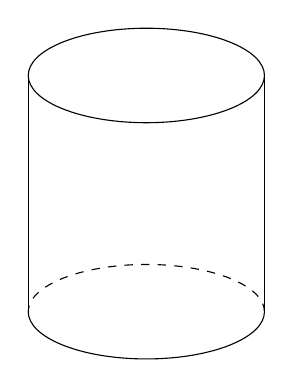
\begin{tikzpicture}
    \newcommand{\size}{1.5}
    \draw (-\size,0) arc (180:360:{\size} and 0.6);
    \draw[dashed] (\size,0) arc (0:180:{\size} and 0.6);
    \draw (-\size,\size+\size) arc (180:360:{\size} and 0.6);
    \draw (\size,\size+\size) arc (0:180:{\size} and 0.6);
    \draw (-\size,0)--(-\size,\size+\size);
    \draw (\size,0)--(\size,\size+\size);
    %\draw[dashed] (\size,0)--(0,0)--(0,\size+\size);
    %\node at (0,-\size+\size/4) {\textit{A right cylinder.}};
    %\filldraw (0,0) circle (1pt);
    %\node at (\size/2,\size/8) {$r$};
    %\node at (\size/6,\size) {$h$};
    \end{tikzpicture}
    \hspace{1.5cm}
    %\textit{A right cylinder.}
    %\\[1\baselineskip]
    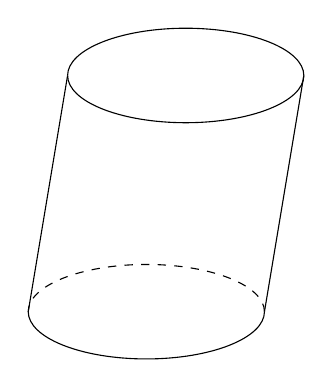
\begin{tikzpicture}
    \newcommand{\size}{1.5}
    \newcommand{\slant}{0.5}
    \draw (-\size,0) arc (180:360:{\size} and 0.6);
    \draw[dashed] (\size,0) arc (0:180:{\size} and 0.6);
    \draw (-\size+\slant,\size+\size) arc (180:360:{\size} and 0.6);
    \draw (\size+\slant,\size+\size) arc (0:180:{\size} and 0.6);
    \draw (-\size,0)--(-\size+\slant,\size+\size);
    \draw (\size,0)--(\size+\slant,\size+\size);
    %\draw[dashed] (\size,0)--(0,0);
    %\draw[dashed] (\size+\slant,0)--(\size+\slant,\size+\size);
    %\node at (0,-\size+\size/4) {\textit{An oblique cylinder.}};
    %\filldraw (0,0) circle (1pt);
    %\node at (\size/2,\size/8) {$r$};
    %\node at (\slant+\size+\size/6,\size/5+\size/5+\size/5+\size/5) {$h$};
    \end{tikzpicture}
\end{center}

\begin{fact}[Rearranging Principle]
If you can rearrange a solid into another solid, the two solids have the same volume.
\end{fact}

This means that if you have a rectangular prism attached to another, you can just find the sum of the volumes of the two rectangular prisms to find the volume of the joined solid. Similar methods apply for other combinations of solids.

\subsection{Surface Area}
Surface area is surprisingly hard to define formally. Intuitively, it is just the area of the surfaces.

\begin{fact}[Additivity]
The surface area of an object is the sum of the surface area of its parts.
\end{fact}

\begin{fact}[Surface Area of Flat Shapes]
The surface area of a flat shape is the same as the area of the flat shape.
\end{fact}

\begin{fact}[Straight Lines]
If part of the surface consists of lines, then the surface area of that part can be found by integrating the lengths of the lines.
\end{fact}
As an example, consider the side of a cylinder or the lines joining the apex of a cone to the circumference of its base.

\begin{fact}[Curves]
If part of the surface consists of curves, then the surface area of that part can be found by integrating the lengths of the curves.
\end{fact}
This will be useful for spheres.

\section{Prisms and Cylinders}

Prisms and cylinders are similar in that a cylinder is analogous to a prism with a continuous base. We also discuss some specific prisms, such as cubes, rectangular prisms, and parallelepipeds.

\subsection{Prisms and Cylinders}
We define a prism and a cylinder.

\begin{defi}[Prism]
A prism is a solid with two congruent parallel bases with parallelograms for the side faces.
\end{defi}

An equivalent definition is that a prism is a solid with two bases that can be translated to each other.

\begin{defi}[Cylinder]
A cylinder is a solid with two parallel circles as bases.
\end{defi}

\begin{defi}[Right Prism and Cylinder]
A prism or cylinder is considered \textit{right} if a line joining two corresponding points on the two bases is perpendicular to both bases.
\end{defi}

Unless otherwise specified, prisms and cylinders are right. Regardless, the volume formulas \textit{always} hold.

\begin{center}
    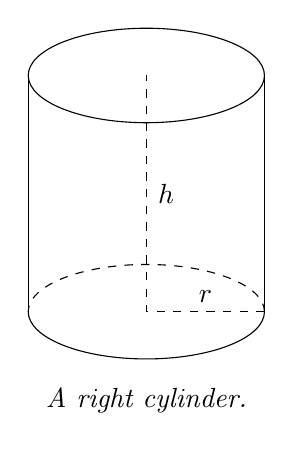
\begin{tikzpicture}
    \newcommand{\size}{1.5}
    \draw (-\size,0) arc (180:360:{\size} and 0.6);
    \draw[dashed] (\size,0) arc (0:180:{\size} and 0.6);
    \draw (-\size,\size+\size) arc (180:360:{\size} and 0.6);
    \draw (\size,\size+\size) arc (0:180:{\size} and 0.6);
    \draw (-\size,0)--(-\size,\size+\size);
    \draw (\size,0)--(\size,\size+\size);
    \draw[dashed] (\size,0)--(0,0)--(0,\size+\size);
    \node at (0,-\size+\size/4) {\textit{A right cylinder.}};
    %\filldraw (0,0) circle (1pt);
    \node at (\size/2,\size/8) {$r$};
    \node at (\size/6,\size) {$h$};
    \end{tikzpicture}
    \hspace{1.5cm}
    %\textit{A right cylinder.}
    %\\[1\baselineskip]
    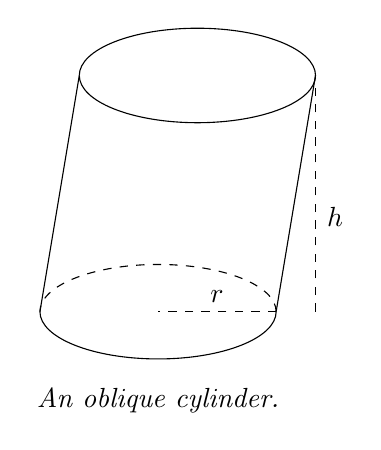
\begin{tikzpicture}
    \newcommand{\size}{1.5}
    \newcommand{\slant}{0.5}
    \draw (-\size,0) arc (180:360:{\size} and 0.6);
    \draw[dashed] (\size,0) arc (0:180:{\size} and 0.6);
    \draw (-\size+\slant,\size+\size) arc (180:360:{\size} and 0.6);
    \draw (\size+\slant,\size+\size) arc (0:180:{\size} and 0.6);
    \draw (-\size,0)--(-\size+\slant,\size+\size);
    \draw (\size,0)--(\size+\slant,\size+\size);
    \draw[dashed] (\size,0)--(0,0);
    \draw[dashed] (\size+\slant,0)--(\size+\slant,\size+\size);
    \node at (0,-\size+\size/4) {\textit{An oblique cylinder.}};
    %\filldraw (0,0) circle (1pt);
    \node at (\size/2,\size/8) {$r$};
    \node at (\slant+\size+\size/6,\size/5+\size/5+\size/5+\size/5) {$h$};
    \end{tikzpicture}
\end{center}

\begin{theo}[Volume of a Prism]
The volume of a prism with a base of area $B$ and a height of $h$ is $Bh.$
\end{theo}

\begin{theo}[Volume of a Cylinder]
The volume of a cylinder with a base if area $B$ and a height of $h$ is $Bh.$
\end{theo}
An alternative formulation of this is that the volume of a cylinder with radius $r$ and height $h$ is $\pi r^2h.$

We prove both volume formulas in one fell swoop.

\begin{pro}
Let the reference plane be one of the bases. Then note that the cross-section always has area $B$ over a height of $h.$ Let $k$ be the distance of the cross-section from the base. Then the volume is $\int\limits_{0}^h Bkdk=Bh.$
\end{pro}

\begin{theo}[Surface Area of a Right Cylinder]
The surface area of a right cylinder with radius $r$ and height $h$ is $2\pi r^2+2\pi rh.$
\end{theo}

\begin{pro}
The two faces have area $\pi r^2$ each, and the lateral surface area (surface area of the sides) can be found by integrating the circumference of the base about the height. So the lateral surface area is $\int\limits_0^h 2\pi rdx=2\pi rh.$ Thus the total surface area is $2\pi r^2+2\pi rh.$
\end{pro}

\subsection{Cubes and Rectangular Prisms}

We discuss cubes and rectangular prisms.

\begin{defi}[Cube]
A cube is a solid with $6$ square faces.
\begin{center}
% \usetikzlibrary{positioning,calc}
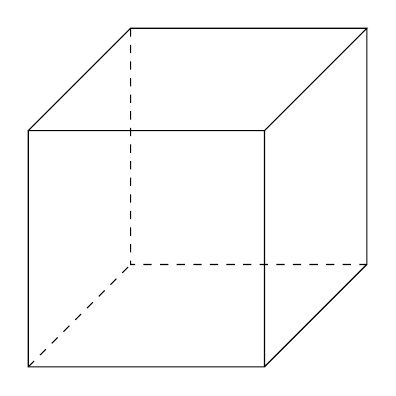
\begin{tikzpicture}
            \newcommand{\side}{3}
            \newcommand{\otherside}{1.3}
            \draw[dashed] (\otherside,\side+\otherside) -- (\otherside,\otherside) -- (\side+\otherside,\otherside)
            (0,0) -- (\otherside,\otherside);
            \draw (0,0) rectangle (\side,\side)
            (0,\side) -- (\otherside,\otherside+\side) -- (\otherside+\side,\otherside+\side) -- (\side,\side)
            (\otherside+\side,\otherside+\side) -- (\otherside+\side,\otherside) -- (\side,0);
\end{tikzpicture}
\end{center}
\end{defi}

\begin{theo}[Volume of a Cube]
The volume of a cube with side length $x$ is $x^3.$
\end{theo}

\begin{pro}
A cube is a prism with base area $x^2$ and height $x,$ so its area is $x^3.$
\end{pro}

\begin{theo}[Surface Area of a Cube]
The surface area of a cube with side length $x$ is $6x^2.$
\end{theo}

\begin{pro}
There are six faces, and each face has surface area $x^2.$ Thus the total surface area is $6x^2.$
\end{pro}

\begin{defi}[Rectangular Prism]
A rectangular prism is a prism with rectangular bases.
\begin{center}
% \usetikzlibrary{positioning,calc}
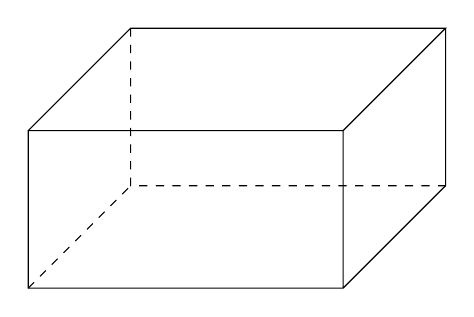
\begin{tikzpicture}
            \newcommand{\wide}{3}
            \newcommand{\figlength}{4}
            \newcommand{\high}{2}
            \newcommand{\otherside}{1.3}
            \draw[dashed] (\otherside,\high+\otherside) -- (\otherside,\otherside) -- (\figlength+\otherside,\otherside)
            (0,0) -- (\otherside,\otherside);
            \draw (0,0) rectangle (\figlength,\high)
            (0,\high) -- (\otherside,\otherside+\high) -- (\otherside+\figlength,\otherside+\high) -- (\figlength,\high)
            (\otherside+\figlength,\otherside+\high) -- (\otherside+\figlength,\otherside) -- (\figlength,0);
\end{tikzpicture}
\end{center}
\end{defi}

In this chapter, a rectangular prism will always refer to a \textit{right} rectangular prism. Unless otherwise specified, rectangular prisms are right. This is generally true in competitions as well.

\begin{theo}[Volume of a Right Rectangular Prism]
The volume of a rectangular prism with side lengths $l,w,h$ is $lwh.$
\end{theo}

\begin{pro}
The base has area $lw$ and the height is $h,$ so the volume is $lwh.$
\end{pro}

\begin{theo}[Surface Area of a Right Rectangular Prism]
The surface area of a rectangular prism with side lengths $l,w,h$ is $2(lw+wh+hl).$
\end{theo}

\begin{pro}
There are two faces with the dimensions $l\times w,$ $w\times h,$ and $h\times l.$ Multiplication and addition finish.
\end{pro}

\begin{exam}
Three faces of a rectangular prism have areas $6,10,15.$ Find the volume of the rectangular prism.
\end{exam}
\begin{sol}
Let the side lengths be $a,b,c.$ Note that
\[ab=6\]
\[bc=10\]
\[ca=15,\]
and the volume of the prism is $abc.$ Multiplying all of the expressions together gives us $(abc)^2=900,$ or $abc=30.$
\end{sol}

\subsection{Parallelepipeds}

\begin{defi}[Parallelepipeds]
A parallelpiped is a solid with $6$ parallelogram faces.
\begin{center}
    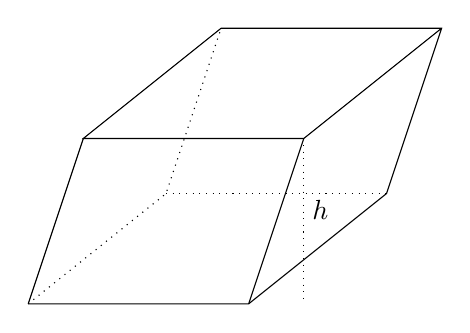
\begin{tikzpicture}[scale=0.7]
\draw (0,0) -- (4,0) -- (6.5,2) -- (7.5,5) -- (3.5,5) -- (1,3) -- (5,3) -- (7.5,5);
\draw (0,0) -- (1,3);
\draw (4,0) -- (5,3);
\draw [dotted] (0,0) -- (2.5,2) -- (3.5,5);
\draw [dotted] (2.5,2)--(6.5,2);
\draw [dotted] (5,3)--(5,0);
\node at (5.3,1.7) {$h$};
\end{tikzpicture}
\end{center}
\end{defi}
Note that all parallelepipeds are prisms.

\begin{theo}[Volume of a Parallelepiped]
The volume of a parallelepiped with a base of area $B$ and height $h$ is $Bh.$
\end{theo}
The surface area of a parallelepiped should also not be too hard to compute, though there is no nice general formula.

\section{Pyramids and Cones}
Pyramids and cones are similar in that a cylinder is analogous to a prism with a continuous base.

\subsection{Pyramids}

\begin{defi}
A pyramid is a solid with a polygonal base whose vertices are all joined to a point not in the plane of the base. This point is called the \textit{apex}.
\begin{center}
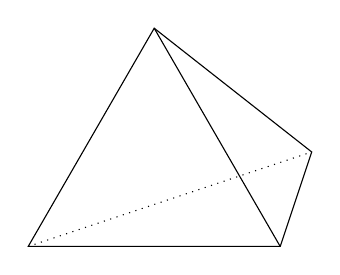
\begin{tikzpicture}[scale=0.8]
\draw (0,0)--(4,0)--(4.5,1.5)--(2,3.46410162)--cycle;
\draw (2,3.46410162)--(4,0);
\draw[dotted] (0,0)--(4.5,1.5);
\end{tikzpicture}
\end{center}
\end{defi}

\begin{theo}[Volume of a Pyramid]
The volume of a pyramid with a base of area $B$ and a height of $h$ is $\frac{Bh}{3}.$
\end{theo}

\begin{pro}
Let the reference plane be the plane through the apex parallel to the base and let $k$ be the distance of the cross-section from the reference plane. (The cross-section lies on the same side of the reference plane as the base.)

Then by similarity, the volume is $\int\limits_0^k B\frac{k^2}{h^2}dk=\frac{B}{h^2}\int\limits_0^k k^2dk=\frac{B}{h^2}\cdot\frac{h^3}{3}=\frac{Bh}{3}.$
\end{pro}

\subsection{Cones}

\begin{defi}
A cone is a solid with a circular base where every point on the base is joined to a point not in the plane of the base. This point is called the \textit{apex}.
\end{defi}

The volume formula is identical to the volume of a pyramid.

\begin{theo}[Volume of a Cone]
The volume of a cone with a base of area $B$ and a height of $h$ is $\frac{Bh}{3}.$ An alternative formulation of this is that the volume of a cone with radius $r$ and height $h$ is $\frac{\pi r^2h}{3}.$
\end{theo}

\begin{pro}
Let the reference plane be the plane through the apex parallel to the base and let $k$ be the distance of the cross-section from the reference plane. (The cross-section lies on the same side of the reference plane as the base.)

Then by similarity, the volume is $\int\limits_0^k B\frac{k^2}{h^2}dk=\frac{B}{h^2}\int\limits_0^k k^2dk=\frac{B}{h^2}\cdot\frac{h^3}{3}=\frac{Bh}{3}.$

To prove the alternate formulation, note that $B=\pi r^2.$
\end{pro}

\begin{defi}[Right and Oblique Cones]
A cone is right if the line joining the center of it bases with the apex is perpendicular to the base, and oblique otherwise.
\end{defi}
Unless otherwise specified, cones are right. This is generally true in competitions as well. Regardless, the volume formula \textit{always} holds.

\begin{center}
    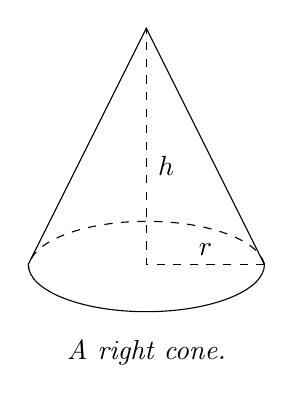
\begin{tikzpicture}
    \newcommand{\size}{1.5}
    \draw (-\size,0) arc (180:360:{\size} and 0.6);
    \draw[dashed] (\size,0) arc (5:180:{\size} and 0.6);
    
    \draw (-\size,0)--(0,\size+\size)--(\size,0);
    \draw[dashed] (\size,0)--(0,0)--(0,\size+\size);
    
    \node at (\size/2,\size/8) {$r$};
    \node at (\size/6,\size-\size/6) {$h$};
    
    \node at (0,-\size+\size/4) {\textit{A right cone.}};
    \end{tikzpicture}
    \hspace{1.5cm}
    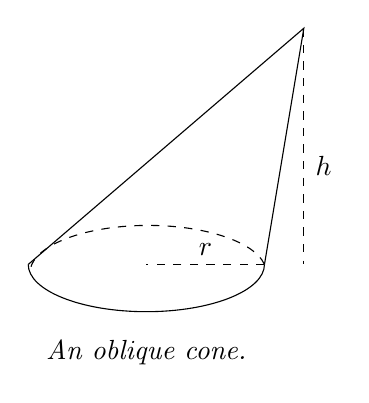
\begin{tikzpicture}
    \newcommand{\size}{1.5}
    \newcommand{\slant}{2}
    \draw (-\size,0) arc (180:360:{\size} and 0.6);
    \draw[dashed] (\size,0) arc (10:180:{\size} and 0.6);
    
    \draw (-\size,0)--(\slant,\size+\size)--(\size,0);
    \draw[dashed] (\size,0)--(0,0);
    \draw[dashed] (\slant,\size+\size)--(\slant,0);
    
    \node at (\size/2,\size/8) {$r$};
    \node at (\slant+\size/6,\size-\size/6) {$h$};
    
    \node at (0,-\size+\size/4) {\textit{An oblique cone.}};
    \end{tikzpicture}
\end{center}

\begin{theo}[Surface Area of a Right Cone]
The surface area of a cone with radius $r$ and height $h$ is $\pi r^2+2\pi r\sqrt{r^2+h^2}.$
\end{theo}

\begin{pro}
The area of the base is $\pi r^2,$ and the lateral surface area can be found by integrating the slant height over the circumference. The lateral surface area is $\int\limits_{0}^{2\pi r}\sqrt{r^2+h^2}dx=2\pi r\sqrt{r^2+h^2.}$ (Note that the slant height is $\sqrt{r^2+h^2}$ by the Pythagorean Theorem.) Adding gives $\pi r^2+2\pi r\sqrt{r^2+h^2}.$
\end{pro}

The surface area of an oblique cone is surprisingly hard to find.

\section{Spheres}

Spheres are the $3$ dimensional version of circles.
\begin{defi}[Sphere]
A sphere is the locus of points in space equidistant from a certain point. This point is called the center.
\begin{center}
    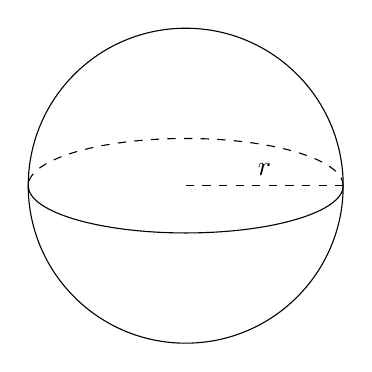
\begin{tikzpicture}
%  \shade[ball color = gray!40, opacity = 0.4] (0,0) circle (2cm);
  \draw (0,0) circle (2cm);
  \draw (-2,0) arc (180:360:2 and 0.6);
  \draw[dashed] (2,0) arc (0:180:2 and 0.6);
%  \fill[fill=black] (0,0) circle (1pt);
  \draw[dashed] (0,0 ) -- node[above]{$r$} (2,0);
\end{tikzpicture}
\end{center}
\end{defi}

\begin{theo}[Volume of a Sphere]
The volume of a sphere with radius $r$ is $\frac{4\pi r^3}{3}.$
\end{theo}

\begin{pro}
Instead we prove the volume of a hemisphere is $\frac{2\pi r^3}{3}.$ Let the reference plane be the base of the hemisphere.

Then let the cross-section have a distance of $k$ from the base. Then by the Pythagorean Theorem, the radius of the cross-section is $\sqrt{r^2-k^2},$ so the area of the cross-section is $\pi(r^2-k^2).$ Thus the volume is \[\int\limits_{0}^{r}\pi(r^2-k^2)dk=\pi r^3-\pi \int\limits_{0}^{r}k^2dk=\pi r^3-\frac{\pi r^3}{3}=\frac{2\pi r^3}{3}.\]
Multiplying by $2$ implies that the volume of the sphere is $\frac{4\pi r^3}{3}.$
\end{pro}

\begin{theo}[Surface Area of a Sphere]
The surface area of a sphere with radius $r$ is $4\pi r^2.$
\end{theo}

To prove this, we first make an observation of what the surface area of the sphere is.

\begin{fact}[Surface Area of a Sphere]
The surface area of a sphere is the integral of the circumferences of all cross-sections made with planes parallel to a certain reference plane.
\end{fact}

Now we can explicitly integrate.

\begin{pro} % THIS IS WRONG: FIX PLS
We instead prove that the surface area of a hemisphere, not counting the base, is $2\pi r^2.$

We integrate about the arc of the circumference. Let $\theta$ be the angle a point on the cross-section forms with the radius containing the foot from the point onto the base. Then we integrate about $t=r\theta.$ Note integrating the circumferences gives
\[\int_0^{\frac{\pi r}{2}}2\pi r\cos\frac{t}{r}dt=2\pi r^2.\]
Multiplying by $2$ implies that the surface area of the sphere is $4\pi r^2.$

\begin{center}
    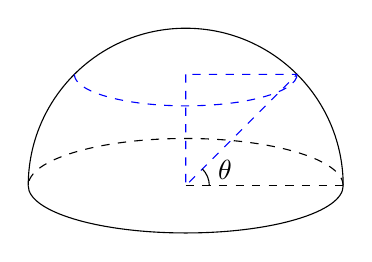
\begin{tikzpicture}
%  \shade[ball color = gray!40, opacity = 0.4] (0,0) circle (2cm);
  \draw (2,0) arc (0:180:2);
  \draw [blue,dashed](-1.41421356,1.41421356) arc (180:360:1.41421356 and 0.4);
  \draw (-2,0) arc (180:360:2 and 0.6);
\draw[dashed] (2,0) arc (0:180:2 and 0.6);
\draw[blue,dashed] (0,1.41421356)--(0,0)--(1.41421356,1.41421356)--cycle;
\draw[dashed] (0,0)--(2,0);
\draw (0.3,0) arc (0:45:0.3);
\node at (0.5,0.2) {$\theta$};
%  \fill[fill=black] (0,0) circle (1pt);
%  \draw[dashed] (0,0 ) -- node[above]{$r$} (2,0);
\end{tikzpicture}
\end{center}
\end{pro}

\section{Cross-sections}

\begin{defi}[Cross-section]
A cross-section of a solid is the intersection of the solid with a plane.
\end{defi}

The word “solid” implies that the interior of the object is part of it.

\begin{theo}[Cross-section of a Sphere]
The cross-section of a sphere is a circle.
\end{theo}

You can also take cross-sections of a cube and a cone. The former is used sometimes in math competitions, and the latter produces a shape known as a \textit{conic}.

\begin{theo}[Cross-section of a Cube]
The cross-section of a cube can be a triangle, quadrilateral, pentagon, or hexagon.
\end{theo}

The heuristical reason this is true is because a cube has $6$ faces, and the plane can intersect the cube at any $6$ of those faces. It's not too hard to construct any polygon with less than $7$ sides.

Sometimes the entire problem is reduced significantly or just solved by taking the correct cross section.

\begin{exam}
Inside a cone of radius $5$ and height $12$ there is a sphere inscribed. What is its radius?
\end{exam}
\begin{sol}
Here is a walkthrough of the solution.
\begin{enumerate}
    \item Take a cross section through the apex of the cone perpendicular to the base.
    
    \item Now you have a triangle and its incircle. Finish with $[ABC]=rs.$
\end{enumerate}
\end{sol}

\begin{exam}[AMC 10A 2019/21]
A sphere with center $O$ has radius 6. A triangle with sides of length $15$, $15$, and $24$ is situated in space so that each of its sides are tangent to the sphere. What is the distance between $O$ and the plane determined by the triangle?
\end{exam}
\begin{sol}
Here is a walkthrough of the solution.
\begin{enumerate}
    \item This is not actually a 3D geometry problem.

    \item Take a cross section of the sphere with the triangle.
    
    \item Use $[ABC]=rs$ to figure out the radius of the cross-section.
    
    \item Finish with the Pythagorean Theorem.
\end{enumerate}
\end{sol}

\section{Miscellaneous Configurations}
Here are some examples of miscellaneous techniques that can help solve 3D geometry problems.

\subsection{Pythagorean Theorem}
The Pythagorean Theorem still holds in 3 dimensions, and can be generalized to a 3 dimensional version by applying the two dimensional version twice.

\begin{exam}
Consider unit cube $ABCDEFGH,$ where $ABCD$ and $EFGH$ are opposite faces and $AG,BH,CE,DF$ are space diagonals. Find the area of triangle $AFH.$
\end{exam}

\begin{sol}
Note that $AF=FH=HA=\sqrt{2}$ by the Pythagorean Theorem, so the area is $\frac{(\sqrt{2})^2\sqrt{3}}{4}=\frac{\sqrt{3}}{2}.$
\end{sol}

\subsection{Tangent Spheres}
For problems with tangent spheres, remember the following fact.
\begin{fact}[Tangency Point is Collinear with Centers]
If two spheres with centers $O_1,O_2$ are tangent at $T,$ then $O_1,O_2,T$ are collinear.
\end{fact}
This implies the following corollary.
\begin{fact}[Distance Between Centers]
Say two spheres $\Gamma_1,\Gamma_2$ with centers $O_1,O_2$ and radii $r_1,r_2$ are tangent at $T.$ Then
\[\begin{cases}
O_1O_2=r_1+r_2 \text{ if } \Gamma_2 \text{ is externally tangent to } \Gamma_1 \\
O_1O_2=r_1-r_2 \text{ if } \Gamma_2 \text{ is internally tangent to } \Gamma_1.
\end{cases}\]
\end{fact}
Using this in conjunction with the Pythagorean Theorem is enough to solve almost all problems with tangent spheres.
\begin{exam}[AMC 12A 2004/22]
Three mutually tangent spheres of radius $1$ rest on a horizontal plane. A sphere of radius $2$ rests on them. What is the distance from the plane to the top of the larger sphere?
\end{exam}
\begin{sol}
Let's label some points. Let the centers of the unit spheres be $O_1,O_2,O_3,$ let the center of the sphere of radius $2$ be $O,$ and let the foot of the perpendicular from $O$ to $O_1O_2O_3$ be $P.$ Note that $O_1O_2O_3$ is parallel to the horizontal plane with a distance of $1.$

Note that $\triangle O_1O_2O_3$ is equilateral with side length $2,$ and by symmetry, $P$ must be the center. Thus $PO_1=\frac{2\sqrt{3}}{3}.$ Since $OO_1=3$ by Fact $2,$ $OP=\sqrt{OO_1^2-PO_1^2}=\sqrt{3^2-(\frac{2\sqrt{3}}{3})^2}=\frac{\sqrt{69}}{3}.$

Since the distance from $P$ to the horizontal plane is $1$ and the tip of the sphere with radius $2$ is $2$ above $O,$ the answer is $1+2+\frac{\sqrt{69}}{3}=3+\frac{\sqrt{69}}{3}.$
\begin{center}
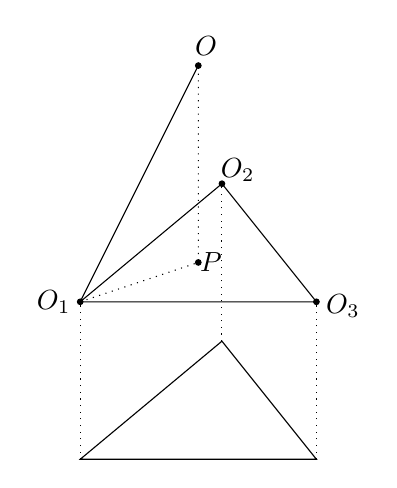
\begin{tikzpicture}
    \draw (0,0)--(1.8,1.5)--(3,0)--cycle; 
    \draw (0,2)--(1.8,3.5)--(3,2)--cycle;
    \draw [dotted] (0,0)--(0,2);
    \draw [dotted] (1.8,1.5)--(1.8,3.5);
    \draw [dotted] (3,0)--(3,2);
    \draw [dotted] (0,2)--(1.5,2.5)--(1.5,5);
    \draw (1.5,5)--(0,2);
    \node at (0,2) [anchor=east] {$O_1$};
    \node at (2,3.4) [anchor=south] {$O_2$};
    \node at (3,1.95) [anchor=west] {$O_3$};
    \node at (1.4,2.5) [anchor=west] {$P$};
    \node at (1.6,5) [anchor=south] {$O$};
    \filldraw (0,2) circle (1pt);
    \filldraw (1.8,3.5) circle (1pt);
    \filldraw (3,2) circle (1pt);
    \filldraw (1.5,2.5) circle (1pt);
    \filldraw (1.5,5) circle (1pt);
\end{tikzpicture}
\end{center}
\end{sol}
Notice that the entire solution was essentially just using the correct setup and the Pythagorean Theorem.

\subsection{Unfolding}
These are problems where you take the shortest path from one point to another on the surface of a solid.

\begin{exam}
Consider a $10\times 10\times 7$ rectangular prism with $A$ as the center of a $10\times 10$ squares and $B$ as a vertex of the opposite $10\times 10$ square. If an ant crawls along the surface of the prism from $A$ to $B,$ what is the length of the shortest path he could take?
\end{exam}

\begin{sol}
Unfold the square and lay it flat with the rectangle containing $B.$ Since the shortest distance between two points is a line, $AB=\sqrt{AP^2+BP^2}=\sqrt{(\frac{10}{2})^2+(\frac{10}{2}+7)^2}=13,$ where $P$ is the foot of the altitude from $A$ to the side of the square whose extension passes through $V.$
\begin{center}
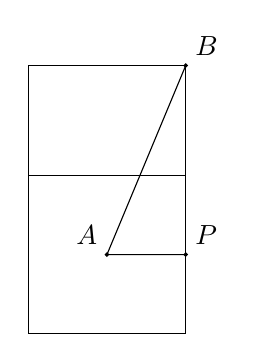
\begin{tikzpicture}[scale=0.2]
\draw (0,0)--(10,0)--(10,17)--(0,17)--cycle;
\draw (0,10)--(10,10);
\draw (10,5)--(5,5)--(10,17);
\filldraw (5,5) circle (3pt) node[anchor=south east] {$A$};
\filldraw (10,5) circle (3pt) node[anchor=south west] {$P$};
\filldraw (10,17) circle (3pt) node[anchor=south west] {$B$};
\end{tikzpicture}
\end{center}
\end{sol}

\section{Summary}

\subsection{Theory}

\begin{enumerate}
\item Prisms and Cylinders

\begin{itemize}
\Item The volume is $Bh.$

\Item The surface area of a cylinder is $2\pi r^2+2\pi rh.$

\Item The volume of a cube is $x^3.$

\Item The surface area of a cube is $6x^2.$

\Item The volume of a right rectangular prism is $lwh.$

\Item The surface area of a right rectangular prism is $2(lw+wh+hl).$
\end{itemize}
\item Pyramids and Cones
\begin{itemize}
\Item The volume is $\frac{Bh}{3}.$

\Item The surface area of a cylinder is 
\end{itemize}
\end{enumerate}

\subsection{Tips and Tricks}
\begin{enumerate}
\item Classifications
\begin{itemize}
\Item Think of prisms and cylinders as one group of solids, pyramids and cones as another, and spheres as their own thing.
\Item The design of this chapter explicitly reflects this.
\end{itemize}
\item Techniques
\begin{itemize}
\Item Think in cross-sections whenever possible.

\Item The Pythagorean Theorem still holds.

\Item Tangent spheres can be reduced to points.

\Item Problems where you find a path along a surface can be solved via unfolding.
\end{itemize}
\end{enumerate}

\pagebreak

\section{Exercises}

\subsection{Check-ins}

\begin{enumerate}
\item Consider a rectangular prism whose base has an area of $40$ and a height of $17.$ What is its volume?

\item Consider a cylinder with diameter $10$ and height $7.$ What is its volume?

\item The net of a 3D figure is composed of 6 congruent squares and has a total area of 216 square inches. When the shape is folded to form a cube, how cubic inches are in its volume?
\begin{center}
    \begin{asy}
    size(5cm);
    draw((0,0)--(4,0)--(4,1)--(0,1)--cycle);
    draw((1,-1)--(2,-1)--(2,2)--(1,2)--cycle);
    draw((3,0)--(3,1));
    \end{asy}
\end{center}

\item The numerical surface area and volume of a sphere are the same. What is the radius of this sphere?

\item Consider two right cylinders $P$ and $Q$ with the same volume. Cylinder $P$ has a radius $30\%$ longer than Cylinder $Q.$ What percent larger is the height of Cylinder $Q$ than that of Cylinder $P?$

\item A right rectangular prism with a volume of $32000$ and a base width of $8$ and a base length of $10.$ When the prism is cut by a plane parallel and equidistant to both bases, what is the combined surface area of the two remaining figures?

\item (AHSME 1996/9) Triangle $PAB$ and square $ABCD$ are in perpendicular planes. Given that $PA = 3, PB = 4$ and $AB = 5$, what is $PD?$

\begin{center}
    \begin{asy}
size(5cm);
    import olympiad;
    real r=sqrt(2)/2;
draw(origin--(8,0)--(8,-1)--(0,-1)--cycle);
draw(origin--(8,0)--(8+r, r)--(r,r)--cycle);
filldraw(origin--(-6*r, -6*r)--(8-6*r, -6*r)--(8, 0)--cycle, white, black);
filldraw(origin--(8,0)--(8,6)--(0,6)--cycle, white, black);
pair A=(6,0), B=(2,0), C=(2,4), D=(6,4), P=B+1*dir(-65);
draw(A--P--B--C--D--cycle);
dot(A^^B^^C^^D^^P);
label("$A$", A, dir((4,2)--A));
label("$B$", B, dir((4,2)--B));
label("$C$", C, dir((4,2)--C));
label("$D$", D, dir((4,2)--D));
label("$P$", P, dir((4,2)--P));
    \end{asy}
\end{center}

\item One dimension of a cube is increased by $1$, another is decreased by $1$, and the third is left unchanged. The volume of the new rectangular solid is $5$ less than that of the cube. What was the volume of the cube?

\item What is the volume of a cube whose surface area is twice that of a cube with volume 1?
\end{enumerate}

\subsection{Problems}

\begin{enumerate}
\item Consider rectangular prism $ABCDEFGH$ with dimensions $1 \times 1 \times \sqrt{3}.$ Let $AE,$ $BF,$ $CG,$ and $DH$ be perpendicular to planes $ABCD$ and $EFGH,$ and let $AE = BF = CG = DH = 1.$ Furthermore, let $AB = 1$ and $BC = \sqrt{3}.$ Find $\angle AGC.$

\item (AMC 12B 2008/18) On a sphere with a radius of $2$ units, the points $A$ and $B$ are $2$ units away from each other. Compute the distance from the center of the sphere to the line segment $AB.$

\item A parallelelepiped has coordinates $(0,0,0),(2,0,0),(1,\sqrt{3},0),(3,\sqrt{3},0)$ for one face and coordinates $(1,0,2),(3,0,2),(2,\sqrt{3},2),(4,\sqrt{3},2)$ for the opposite face. Find its surface area.

\item (AMC 12A 2005/22) A rectangular box $P$ is inscribed in a sphere of radius $r$. The surface area of $P$ is 384, and the sum of the lengths of its 12 edges is 112. What is $r$?

\item (AMC 12B 2005/16) Eight spheres of radius 1, one per octant, are each tangent to the coordinate planes. What is the radius of the smallest sphere, centered at the origin, that contains these eight spheres.

\item Consider two externally spheres $\Gamma_1$ and $\Gamma_2$ with radii $12,r,$ and consider cylinder $\Omega$ with radius $16$ and height $25.$ If $\Gamma_1$ is tangent to a base and the circumference of $\Omega$ and $\Gamma_2$ is tangent to the opposite base and the circumference of $\Omega,$ find $r.$

\item (AMC 10B 2018/10) In the rectangular parallelepiped shown, $AB$ = $3$, $BC$ = $1$, and $CG$ = $2$. Point $M$ is the midpoint of $\overline{FG}$. What is the volume of the rectangular pyramid with base $BCHE$ and apex $M$?
\begin{center}
    \begin{asy}
    import olympiad;
    size(6cm);
pair A = origin;
pair B = (4.75,0);
pair E1=(0,3);
pair F = (4.75,3);
pair G = (5.95,4.2);
pair C = (5.95,1.2);
pair D = (1.2,1.2);
pair H= (1.2,4.2);
pair M = ((4.75+5.95)/2,3.6);
draw(E1--M--H--E1--A--B--E1--F--B--M--C--G--H);
draw(B--C);
draw(F--G);
draw(A--D--H--C--D,dashed);
label("$A$",A,SW);
label("$B$",B,SE);
label("$C$",C,E);
label("$D$",D,W);
label("$E$",E1,W);
label("$F$",F,SW);
label("$G$",G,NE);
label("$H$",H,NW);
label("$M$",M,N);
dot(A);
dot(B);
dot(E1);
dot(F);
dot(G);
dot(C);
dot(D);
dot(H);
dot(M);
label("3",A/2+B/2,S);
label("2",C/2+G/2,E);
label("1",C/2+B/2,SE);
    \end{asy}
\end{center}

\item (AIME I 2020/6) A flat board has a circular hole with radius $1$ and a circular hole with radius $2$ such that the distance between the centers of the two holes is $7.$ Two spheres with equal radii sit in the two holes such that the spheres are tangent to each other. The square of the radius of the spheres is $\tfrac{m}{n},$ where $m$ and $n$ are relatively prime positive integers. Find $m+n.$

\item (AIME 1984/9) In tetrahedron $ABCD$, edge $AB$ has length 3 cm. The area of face $ABC$ is $15\mbox{cm}^2$ and the area of face $ABD$ is $12 \mbox { cm}^2$. These two faces meet each other at a $30^\circ$ angle. Find the volume of the tetrahedron in $\mbox{cm}^3$.

\item (AHSME 1996/28) On a $4\times 4\times 3$ rectangular parallelepiped, vertices $A$, $B$, and $C$ are adjacent to vertex $D$. Find the distance from $D$ to plane $ABC$.
\end{enumerate}

\subsection{Challenges}

\begin{enumerate}
\item (AIME I 2011/12) A sphere is inscribed in the tetrahedron whose vertices are $A = (6,0,0), B = (0,4,0), C = (0,0,2),$ and $D = (0,0,0).$ The radius of the sphere is $m/n,$ where $m$ and $n$ are relatively prime positive integers. Find $m + n.$

\item (AMC 10A 2013/22) Six spheres of radius $1$ are positioned so that their centers are at the vertices of a regular hexagon of side length $2$. The six spheres are internally tangent to a larger sphere whose center is the center of the hexagon. An eighth sphere is externally tangent to the six smaller spheres and internally tangent to the larger sphere. What is the radius of this eighth sphere?

\item (AMC 12B 2004/19) A truncated cone has horizontal bases with radii $18$ and $2$. A sphere is tangent to the top, bottom, and lateral surface of the truncated cone. What is the radius of the sphere?

\item (AIME II 2020/7) Two congruent right circular cones each with base radius $3$ and height $8$ have axes of symmetry that intersect at right angles at a point in the interior of the cones a distance $3$ from the base of each cone. A sphere with radius $r$ lies inside both cones. The maximum possible value for $r^2$ is $\frac mn$, where $m$ and $n$ are relatively prime positive integers. Find $m+n$.

\item (AIME I 2013/7) A rectangular box has width $12$ inches, length $16$ inches, and height $\frac{m}{n}$ inches, where $m$ and $n$ are relatively prime positive integers. Three faces of the box meet at a corner of the box. The center points of those three faces are the vertices of a triangle with an area of $30$ square inches. Find $m+n$.

\item (AIME II 2016/14) Equilateral $\triangle ABC$ has side length $600$. Points $P$ and $Q$ lie outside the plane of $\triangle ABC$ and are on opposite sides of the plane. Furthermore, $PA=PB=PC$, and $QA=QB=QC$, and the planes of $\triangle PAB$ and $\triangle QAB$ form a $120^{\circ}$ dihedral angle (the angle between the two planes). There is a point $O$ whose distance from each of $A,B,C,P,$ and $Q$ is $d$. Find $d$.
\end{enumerate}

\chapter{Hints}

\chapterquote{If anyone tells me it's a mistake to have hope, well then, I'll just tell them they're wrong. And I'll keep telling them 'til they believe! No matter how many times it takes.}{Puella Magi Madoka Magica}

\pgfmathsetseed{2020} % or any other number: sets the random seed

%This is essentially the only way to reliably use loops, in the \makeatletter environment.
\makeatletter
\def\declarenumlist#1#2#3{%
\expandafter\edef\csname pgfmath@randomlist@#1\endcsname{#3}%
\count@\@ne
\loop
\expandafter\edef
\csname pgfmath@randomlist@#1@\the\count@\endcsname
  {\the\count@}
\ifnum\count@<#3\relax
\advance\count@\@ne
\repeat}

\declarenumlist{hintlist}{1}{\value{hintcounter}}

\def\prunelist#1{%
\expandafter\edef\csname pgfmath@randomlist@#1\endcsname
    {\the\numexpr\csname pgfmath@randomlist@#1\endcsname-1\relax}
\count@\pgfmath@randomtemp
\loop
\expandafter\let
\csname pgfmath@randomlist@#1@\the\count@\expandafter\endcsname
\csname pgfmath@randomlist@#1@\the\numexpr\count@+1\relax\endcsname
\ifnum\count@<\csname pgfmath@randomlist@#1\endcsname\relax
\advance\count@\@ne
\repeat}
\makeatother

% Print the hints
\begin{enumerate}
\small
\itemsep2pt
\setcounter{hindex}{0}%
\whiledo{\value{hindex} < \value{hintcounter}}{%
 \addtocounter{hindex}{1}%
 \pgfmathrandomitem\z{hintlist}
 \gethint{\z}
 \prunelist{hintlist}
 }
\end{enumerate}

\chapter{Solutions}

\chapterquote{Regret your helplessness, and feel despair.}{Psycho-Pass}

\pgfmathsetseed{2020} % or any other number: sets the random seed

%This is essentially the only way to reliably use loops, in the \makeatletter environment.
\makeatletter
\def\declarenumlist#1#2#3{%
\expandafter\edef\csname pgfmath@randomlist@#1\endcsname{#3}%
\count@\@ne
\loop
\expandafter\edef
\csname pgfmath@randomlist@#1@\the\count@\endcsname
  {\the\count@}
\ifnum\count@<#3\relax
\advance\count@\@ne
\repeat}

\declarenumlist{sollist}{1}{\value{solcounter}}

\def\prunelist#1{%
\expandafter\edef\csname pgfmath@randomlist@#1\endcsname
    {\the\numexpr\csname pgfmath@randomlist@#1\endcsname-1\relax}
\count@\pgfmath@randomtemp
\loop
\expandafter\let
\csname pgfmath@randomlist@#1@\the\count@\expandafter\endcsname
\csname pgfmath@randomlist@#1@\the\numexpr\count@+1\relax\endcsname
\ifnum\count@<\csname pgfmath@randomlist@#1\endcsname\relax
\advance\count@\@ne
\repeat}
\makeatother
\begin{enumerate}
\small
\itemsep2pt
\setcounter{sindex}{0}%
\whiledo{\value{sindex} < \value{solcounter}}{%
 \addtocounter{sindex}{1}%
 \pgfmathrandomitem\z{sollist}
 \getsol{\z}
 \prunelist{sollist}
 }
\end{enumerate}

\end{document}